\documentclass{article}

\usepackage[top=3cm, bottom=3cm, left=3cm,right=3cm]{geometry}
\usepackage[colorinlistoftodos]{todonotes}
\usepackage{graphicx}
\usepackage{amssymb}
\usepackage{amsmath}
\usepackage{bbm}
\usepackage{todonotes}
\usepackage{pdflscape}
\usepackage{caption}
\usepackage{subcaption}
\usepackage[T1]{fontenc}
\usepackage[utf8]{inputenc}
\usepackage{authblk}
\usepackage{pdfpages}
\usepackage{setspace} 
\usepackage{booktabs}
\usepackage{longtable}
\usepackage{float}
\usepackage{tikz}
\usepackage[colorlinks=true,citecolor=blue, linkcolor=blue]{hyperref}
\usepackage{multirow}
\usepackage{todonotes}
\setlength{\tabcolsep}{5pt}
%%\setlength{\parindent}{0pt}
\usepackage[parfill]{parskip}
\renewcommand{\arraystretch}{1.5}

\renewcommand\Affilfont{\itshape\footnotesize}
\def\ci{\perp\!\!\!\perp}

\renewcommand\Affilfont{\itshape\footnotesize}
\linespread{1.5}

% \usepackage{lineno}
% \linenumbers

% Nature Bibliography style
\usepackage[backend=biber,style=nature]{biblatex}
\addbibresource{library.bib} 

%%%%%%%%%%%%%
%%% Title %%%
%%%%%%%%%%%%%
\title{District-level male medical and traditional circumcision coverage and unmet need in sub-Saharan Africa}

\author{}
\date{}

%%%%%%%%%%%%%%%%%%%%%%%%%%%%%%%%%%%%%%%%%%%%%%%%%%%%%%%%%%%%%%%%%%
%%%%%%%%%%%%%%%%%%%%%%%%%%%%%%%%%%%%%%%%%%%%%%%%%%%%%%%%%%%%%%%%%%
%%%%%%%%%%%%%%%%%%%%%%%%%%%%%%%%%%%%%%%%%%%%%%%%%%%%%%%%%%%%%%%%%%

\begin{document}

%%%%%%%%%%%%%%%%%%%%%%%%%%%%%%%%%%%%%%%%%%%%%%%%%%%%%%%%%%%%%%%%%%
%%%%%%%%%%%%%%%%%%%%%%%%%%%%%%%%%%%%%%%%%%%%%%%%%%%%%%%%%%%%%%%%%%
%%%%%%%%%%%%%%%%%%%%%%%%%%%%%%%%%%%%%%%%%%%%%%%%%%%%%%%%%%%%%%%%%%

\maketitle

\vspace{-1cm}

Patrick O'Toole\textsuperscript{1,2},
Matthew L. Thomas\textsuperscript{1,3,4},
Oliver Stevens\textsuperscript{1},
Kevin Lam\textsuperscript{1,5},
Katharine Kripke\textsuperscript{6},
Rachel Esra\textsuperscript{1},
Ian Wanyeki\textsuperscript{7},
Lycias Zembe\textsuperscript{7},
Jeffrey W. Imai-Eaton\textsuperscript{1,8} \\
\smallskip

\textbf{1} MRC Centre for Global Infectious Disease Analysis, School of Public Health, Imperial College London, London, United Kingdom\\
\textbf{2} Department of Mathematical Sciences, University of Bath, Bath, United Kingdom\\
\textbf{3} Department of Earth and Environmental Sciences, University of Manchester, Manchester, United Kingdom\\
\textbf{4} National Centre for Atmospheric Sciences, University of Manchester, Manchester, United Kingdom\\
\textbf{5} Department of Statistics, University of British Columbia, Vancouver, Canada\\
\textbf{6} Avenir Health, Washington, District of Columbia, United States of America\\
\textbf{7} Joint United Nations Programme on HIV/AIDS (UNAIDS), Geneva, Switzerland\\
\textbf{8} Center for Communicable Disease Dynamics, Department of Epidemiology, Harvard T.H. Chan School of Public Health, Boston, Massachusetts, United States of America\\

\smallskip

* Corresponding Author Email

\clearpage

\begin{abstract}
  \noindent \textbf{Background} \\
  \noindent In 2016, UNAIDS developed a Fast-Track strategy that targeted 90\% coverage
  male circumcision (MC) among men aged 10-29 years by 2021 in priority countries in sub-Saharan 
  Africa (SSA) to reduce HIV incidence. There is substantial variation across subnational 
  regions within countries in both traditional male circumcision (TMC) practices and progress
  towards implementation of voluntary medical male circumcision (VMMC). Tracking progress and
  remaining gaps towards VMMC HIV prevention targets requires detailed district-level circumcision
  coverage data.

  \noindent \textbf{Methods} \\
  \noindent We analysed self-reported data on male circumcision from 
  123
  nationally representative household surveys conducted in 34 SSA countries between 2006 and 2020.
  A spatio-temporal Bayesian competing-risks time-to-event model was used to estimate rates of traditional and medical circumcision by age, location, and time.
  Circumcision coverage in 2020 was projected assuming continuation of estimated age-specific rates, with probabilistic uncertainty.

  \noindent \textbf{Results} \\
  \noindent Across 34 countries, from 2006 to 2020 an estimated 121.943 million men (95\% CI 107.021 - 141.729 million) were newly circumcised, of whom 60.732 million men (45.779 - 85.927 million) were medically circumcised, and 33.519 million men (27.143 - 37.422 million) traditionally circumcised. In 2020, MC coverage among men 10-29 years ranged from 34.31\% (32.39\% - 36.98\%) in Zimbabwe to 100\% (100\% - 100\%) in Niger.
  MMC coverage ranged from 20.55\% (17.62\% - 24.99\%) in Benin to 79.63\% (77.9\% - 81.38\%) in Sierra Leone, and TMC coverage from 0.63\% (0.5\% - 0.78\%) in Eswatini to 75.46\% (71.71\% - 78.64\%) in Benin.
  The largest increase in MMC coverage was in Lesotho Lesotho from 11.53\% to 66.9\%. 
  Within countries, the median difference in MC coverage between the districts with lowest and highest coverage was 31.78\% with the smallest variation in Niger (99.99\% to 100\%) and largest in Zambia (9.2\% to 99.94\%). 
  In VMMC priority countries, 25.474 million men aged 10-29 need to be circumcised to reach 90\% coverage in VMMC priority countries, while 22.282 million circumcisions amongst 15-49 year olds are needed to reach 80\% coverage.
  
  \noindent \textbf{Conclusions} \\
  \noindent VMMC programmes have made substantial, but uneven, progress towards male circumcision targets. Granular district and age-stratified data provide information for focusing further programme implementation.

\end{abstract}

\newpage


%%%%%%%%%%%%%%%%%%%%%%%%%%%%%%%%%%%%%%%%%%%%%%%%%%%%%%%%%%%%%%%%%%
%%%%%%%%%%%%%%%%%%%%%%%%%%%%%%%%%%%%%%%%%%%%%%%%%%%%%%%%%%%%%%%%%%
%%%%%%%%%%%%%%%%%%%%%%%%%%%%%%%%%%%%%%%%%%%%%%%%%%%%%%%%%%%%%%%%%%

\section{Introduction}

%%%%%%%%%%%%%%%%%%%%%%%%%%%%%%%%%%%%%%%%%%%%%%%%%%%%%%%%%%%%%%%%%%
%%%%%%%%%%%%%%%%%%%%%%%%%%%%%%%%%%%%%%%%%%%%%%%%%%%%%%%%%%%%%%%%%%
%%%%%%%%%%%%%%%%%%%%%%%%%%%%%%%%%%%%%%%%%%%%%%%%%%%%%%%%%%%%%%%%%%

The HIV epidemic continues to be a public health priority, with the Joint United Nations Programme on HIV/AIDS (UNAIDS) estimating that over 25 million people live with HIV across sub-Saharan Africa in 2022, with over 650,000 new infections that year \cite{UNAIDSStats}. To achieve the the global community's ambitious goals of ending the AIDS public health crisis by 2030, more work will need to be done \cite{UNAIDSStrategy}. Among the numerous interventions available, voluntary medical male circumcision (VMMC) has emerged as a powerful and cost-effective intervention to reduce HIV incidence \cite{bansi2023cost} with it estimated to reduce male-to-female transition of HIV by 60\% \cite{gray2007male, bailey2007male, auvert2005randomized, gray2012effectiveness, grund2017association}. Furthermore, other research has shown that VMMC can decrease the risk of male-to-male transmission of HIV \cite{pintye2019benefits}, and reduce the transmission of other sexually transmitted infections \cite{tobian2009male}. 

In 2007, the World Health Organization (WHO) and UNAIDS recommended a scale-up in male circumcision coverage for HIV prevention in fifteen countries across Central and Western Africa with a high HIV incidence and low circumcision coverage: Botswana, Eswatini, Ethiopia, Kenya, Lesotho, Malawi, Mozambique, Namibia, Rwanda, South Africa, South Sudan Tanzania, Uganda, Zambia, and Zimbabwe \cite{UNAIDSJoint, davis2018progress, WHOVoluntary2}. UNAIDS' aim was to reach 90\% circumcision coverage among adolescent boys and young men aged 10--29 years by 2021 \cite{WHOFramework}. As a result, over XX\todo{Find this number and cite} million VMMCs have been conducted in these priority countries between 2007 and 2022 with the support of national governments as well as international organisations such as US President’s Emergency Plan for AIDS Relief (PEPFAR). 

There is a need to provide comprehensive \todo{Want to make point that TMC is decreasing in this para, but don't have a reference. Paddy said there was, check with him.} and accurate estimates of male circumcision coverage across all ages, over time, across sub-Saharan Africa to (i) aid VMMC programmes planning, delivery, target setting and checking target attainment and (ii) to evaluate the impacts of VMMC campaigns on HIV incidence. However, this is complex task, as despite the upscaling in medical male circumcision (MMC) being a recent phenomenon, it has been long been practised as part of traditional male initiation ceremonies in many African countries. The coverage and provision of traditional male circumcision (TMC) can vary considerably and is mainly influenced by community, religious, ethnic and cultural led values. For example, in South Africa, TMC coverage ranged from 5.3\% in KwaZulu-Natal to 48.9\% in Eastern Cape among 15-49 year olds, with the average age of circumcision varying from 12.2 years in Limpopo to 20.4 in Western Cape \cite{thomas2024substantial}. \todo{Should I add a national comparison from the results?} TMCs conducted during male initiation ceremonies are often performed using non-medical methods non-clinical settings by a traditional practitioner with no formal medical training \cite{drain2006male, wilcken2010traditional, weiss2000male}. The evidence that TMC provides the same HIV prevention benefits as MMC is mixed, as TMC may not involve a complete circumcision in some populations \cite{WHOTraditional, shaffer2007protective, bailey2008male}.  

There have been a number of recent approaches to estimate coverage of circumcision in sub-Saharan Africa \cite{cork2020mapping, kripke2016age, kripke2016cost, thomas2024substantial}. Cork et al. \cite{cork2020mapping} developed a Bayesian geo-statistical model, which utilizes survey data, to produce annual estimates of total male circumcision coverage sub-nationally in sub-Saharan Africa between 2000 and 2017. This approach is limited cannot provide a full picture of the coverage and provisions of circumcision alone, as the model only produced estimates at the aggregate age range 15–49 years, does not distinguish between circumcision type, and does not track the structured dynamics of circumcision coverage by type within cohorts. Kripke et al. \cite{kripke2016age, kripke2016cost} developed The Decision Makers’ Program Planning Toolkit, Version 2 (DMPPT2), a compartmental model that combines estimates of circumcision coverage from survey data prior to the VMMC scale-up, with information on the reported numbers of VMMCs, to estimate circumcision coverage and unmet need across sub-Saharan Africa in 5-year age groups at a subnational level over time. This approach is also limited as the model does not incorporate data from more recent household surveys (since intervention implementation), does not estimate any uncertainty associated with the circumcision coverage estimates and also does not distinguish by circumcision type. 

Thomas et al. \cite{thomas2024substantial} aimed to address the issues of both models by producing a model to generate region-age-time-type specific probabilities and coverage of male circumcision. The model extended a competing risks time-to-event model which enabled the synthesising of both survey data and programmatic data from VMMC providers. However, this study focused only on South Africa and the model was developed with many local dynamics in the provision to synthesise both data sources. \todo{Jeff-Feel like I need to expand this but not sure how much detaul to give here.}Here, we take a similar approach to Thomas et al. and develop a discrete-time competing risks time-to-event model only using survey data in order to estimate the probabilities and coverage of medical and traditional male circumcision by sub-national area, single-year age, and time along with probabilistic uncertainty. We applied the model to estimate annual probabilities and coverage of circumcision by district in XXX countries across sub-Saharan Africa between 2008 and 2023 in order to quantify gaps in attainment of VMMC targets within priority age groups. 

%%%%%%%%%%%%%%%%%%%%%%%%%%%%%%%%%%%%%%%%%%%%%%%%%%%%%%%%%%%%%%%%%%
%%%%%%%%%%%%%%%%%%%%%%%%%%%%%%%%%%%%%%%%%%%%%%%%%%%%%%%%%%%%%%%%%%
%%%%%%%%%%%%%%%%%%%%%%%%%%%%%%%%%%%%%%%%%%%%%%%%%%%%%%%%%%%%%%%%%%
\newpage
\section{Methods}
\label{sec:orga131cc6}

%%%%%%%%%%%%%%%%%%%%%%%%%%%%%%%%%%%%%%%%%%%%%%%%%%%%%%%%%%%%%%%%%%
%%%%%%%%%%%%%%%%%%%%%%%%%%%%%%%%%%%%%%%%%%%%%%%%%%%%%%%%%%%%%%%%%%
%%%%%%%%%%%%%%%%%%%%%%%%%%%%%%%%%%%%%%%%%%%%%%%%%%%%%%%%%%%%%%%%%%

\subsection{Data}
\label{sec:org020fc8c}

%%%%%%%%%%%%%%%%%%%%%%%%%%%%%%%%%%%%%%%%%%%%%%%%%%%%%%%%%%%%%%%%%%
%%%%%%%%%%%%%%%%%%%%%%%%%%%%%%%%%%%%%%%%%%%%%%%%%%%%%%%%%%%%%%%%%%

The study consisted of 34 sub-Saharan countries, that have conducted surveys that contained information on self-reported circumcision status since 2002: Senegal, Gambia, Guinea, Sierra Leone, Liberia, Mali, Burkina Faso, Côte d’Ivoire, Ghana, Togo, Benin, Niger, Nigeria, Cameroon, Chad, Ethiopia, Gabon, The Republic of the Congo (the Congo), The Democratic Republic of the Congo (DR Congo), Uganda, Kenya, Rwanda, Burundi, Tanzania, Angola, Zambia, Malawi, Mozambique, Zimbabwe, Namibia, Eswatini, Lesotho, South Africa. 
We excluded Equitorial Guinea, Guinea-Bissau and the Central African Republic because they either had no surveys conducted, or, where surveys were available, there was insufficient information available on age at circumcision.

{\color{red} Several major survey series included questions on male circumcision status, namely the Demographic and Health Surveys (DHS), AIDS Indicator Surveys (AIS) Population-based HIV Impact Assessment (PHIA) surveys, Multiple Indicator Cluster Surveys (MICS), and, in the case of South Africa, Human Sciences Research Council (HSRC) surveys.

These surveys provided individual-level data on self-reported circumcision status by male respondents, and from this we estimated circumcision rates over time and by type for the years proceeding each survey. The following questions were of interest:
\begin{itemize}
\item The circumcision status of the male individual,
\item The circumcision provider: whether the individual was circumcised by a health worker/professional, traditional practioner, other or unknown,
\item The circumcision location: whether the individual was circumcised at a health facility, in the home of a health worker/professional, at home, at a ritual site, other or unknown
\item The circumcision year, and
\item The date of birth and age at response and circumcision.
\end{itemize}

The age of respondents was calculated from the century-month-code (CMC) of birth and interview dates.
PHIA surveys did not include a question for circumcision location. Circumcisions performed by a medical professional and/or in a medical setting are categorised as MMC. Otherwise, circumcisions are TMC. Where no data is present on location or provider, circumcision type is treated as "Missing". 

Respondents were located to their districts using masked cluster geocoordinates. Where these coordinates were unavailable, as in several MICS surveys, respondents were located to their admin level 1 area hierarchy, most often corresponding to a province. 

Sub-national populations from WorldPop were used to calculate circumcision coverage from circumcision rates. (reference)}

%%%%%%%%%%%%%%%%%%%%%%%%%%%%%%%%%%%%%%%%%%%%%%%%%%%%%%%%%%%%%%%%%%
%%%%%%%%%%%%%%%%%%%%%%%%%%%%%%%%%%%%%%%%%%%%%%%%%%%%%%%%%%%%%%%%%%

\subsection{Model}
\label{sec:org681dda6}

%%%%%%%%%%%%%%%%%%%%%%%%%%%%%%%%%%%%%%%%%%%%%%%%%%%%%%%%%%%%%%%%%%
%%%%%%%%%%%%%%%%%%%%%%%%%%%%%%%%%%%%%%%%%%%%%%%%%%%%%%%%%%%%%%%%%%

% Following a similar approach to Thomas {\it et al.} \cite{thomas2021multilevel}, we developed a Bayesian hierarchical model with small area estimation methods that uses survey data to estimate the probabilities and coverage of circumcision stratified by region, age, time, and type. We modelled each country independently rather than a model by sub-region or for the whole of sub-Saharan due to computational constraints and we modelled probabilities of circumcision at the organizational level in which the country team has prioritised their program, called the PSNU area level, or the most granular level available in surveys (hereafter called the district-level). 

% In countries where suitable survey information was collected on circumcision type, we consider the following two types of circumcision: (1) circumcisions that occurred in traditional male initiation ceremonies or for other religious or cultural reasons (TMC) and (2) circumcisions for non-traditional reasons and/or HIV prevention that take place in a clinical setting using medical methods (MMC). 

% For the probability of TMC, a key assumption of the \cite{thomas2021multilevel} model was that TMC was constant over time, due to traditional male initiation ceremonies amongst tribal, cultural and religious groups remained stable over time in South Africa however an assumption of a constant probability of TMC might not be feasible everywhere. For example, in some countries the level and practices of TMC have changed through time due to demographic shifts. There has also been a sment of TMCs through MMCs observed, particularly in VMMC priority countries, to ensure HIV prevention efficacy and/or for safety considerations \cite{thomas2021multilevel}. Furthermore, there may also be cases where TMC remains stable and allowing a constant probability of TMC in the competing risks framework will cause a reduction in TMC coverage overall in places where VMMC uptake is high. Here, we consider two models for $\lambda^{\text{TMC}}_{iat}$ in each country: (i) time invariant (i.e. constant over time) and (ii) time variant (i.e. varying over time). The {\it time invariant} probability of TMC was modelled by a logit-linear function with random effects for age, district, as well as an age-district interaction, to allow for different patterns in the age at circumcision across districts. The {\it time variant} was also modelled by a logit-linear function with random effects for age, district, time, as well as age-district and age-time interaction, to allow for different patterns in the age at circumcision across space and time. We did not include a district-time interaction into due to computational constraints. 

% The provision of MMC is highly heterogeneous in sub-Saharan Africa and has changed substantially since 2008, particularly in countries that have programmes to scale-up MMC for HIV prevention. VMMC programmes provide MMCs for HIV prevention to those aged 10 and over, while infant and paediatric medical circumcision often occurs through cultural or religious practices unrelated to scale-up of VMMC for HIV prevention. Due to this, Thomas et al. \cite{thomas2021multilevel} separated the probability of MMC, $\tilde{\lambda}^{\text{MMC}}_{iat}$, into two processes: (i) paediatric circumcision (for those aged 0--9) and (ii) adolescent and adult circumcision (for those aged 10 and over). This ensured that any increase in MMC for those aged 10 and over did not bias the probability of MMC in those under 10 in South Africa. However, this may not be appropriate everywhere, particularly in countries without programmes to upscale MMC coverage. Therefore, we consider two models for the probability of MMC in each country: (i) no cut-off and (ii) paediatric cut off.

% We modelled probability of MMC with {\it no paediatric cut-off} was modelled using logit-linear function with random effects for age, time, and district, and interactions for district-time, age-time, and age-district, to allow for inter-district/time/age variation in circumcision rates. For the probability of MMC with {\it a paediatric cut-off}, the probability of paediatric MMC-nT was modelled using a logit-linear function with random effects for age, district, an age-district interaction, to allow for different practices of paediatric circumcision observed across districts. We assumed that the probability of paediatric MMC-nT was constant over time. The probability of adolescent and adult MMC-nT was also modelled using logit-linear function with random effects for age, time, and district, as well as all the associated two-way interactions to allow for inter-district/time/age variation in circumcision rates. To ensure the probability of MC (i.e. the sum of the probabilities of MMC and TMC) was not larger than one, we applied the probability of TMC before MMC in each time step.

% Whether a country used (i) a time-invariant or time-variant probability of TMC and (i) a paediatric cut-off or no cut-off in the probability of MMC, was decided based on which produced the best within-sample model fit (see Section XX for further details). 

% Some countries did not have any surveys that collected information on the type of circumcision (see Supplementary Material for more detail), so we were unable to conduct an analysis of the probabilities of circumcision by type. For these countries, we consider estimating the probability and coverage of circumcision of any or (unknown) type (MC) only. We used survey data to model the probability of MC directly, using a discrete time-to-event process. We modelled probability of MC using logit-linear function with random effects for age, time, and district, as well as the associated two-way interactions to allow for inter-district/time/age variation in MC rates. 

% We calculated the estimated circumcision coverage by type (MMC/TMC/MC) within each cohort using the cumulative incidence function, which defines the marginal probability (or proportion/coverage of) individuals who were received an MMC, TMC, or MC by district, age and time, whilst accounting for the competing risk of other circumcision type.

% Prior distributions were specified on all model parameters and were specified to allow areas, with little to no data, to borrow district-age-time information on circumcision. Furthermore, we wanted to ensure any correlation in circumcision practices across district, age and time was modelled. We assigned intrinsic conditional autoregressive (ICAR) priors to the district random effects, and penalised B-spline functions on the age random effects. The temporal random effects were assigned one of three potential priors in each country: an autoregressive process of order 1 (AR1), random walk of order 1 (RW1) and random walk of order 2 (RW2). The choice of whether a country uses a AR1, RW1 and RW2 as a temporal prior was chosen depending on which produced the best out-of-sample model fit during model calibration (see Section XX for further details). The age-space, age-time, and space-time interaction terms were modelled as Type IV interactions as defined by Knorr-Held and Leonard, where precision matrices were constructed through Kronecker products. Vague Gaussian priors were assigned to each of the intercepts, and Gaussian priors were specified for all correlation parameters on the logit scale, such that a priori there was 95\% probability that the autocorrelation parameters on AR1 processes were between 0.48 and 0.99 on the real scale. We assigned exponential priors on standard deviations parameters, with the same hyperparameters for the age, district and age-district random effects. For the time, age-time and space-time random effects, the hyperparameters on the exponential priors were decided during model calibration (see Section XX for further details). 

% Technical details of the model are in Supplementary Materials.

%%%%%%%%%%%%%%%%%%%%%%%%%%%%%%%%%%%%%%%%%%%%%%%%%%%%%%%%%%%%%%%%%%
%%%%%%%%%%%%%%%%%%%%%%%%%%%%%%%%%%%%%%%%%%%%%%%%%%%%%%%%%%%%%%%%%%

\subsection{Model specification}
\label{sec:orgaf7fa2a}

%%%%%%%%%%%%%%%%%%%%%%%%%%%%%%%%%%%%%%%%%%%%%%%%%%%%%%%%%%%%%%%%%%
%%%%%%%%%%%%%%%%%%%%%%%%%%%%%%%%%%%%%%%%%%%%%%%%%%%%%%%%%%%%%%%%%%

% In our choice of model specification, we were interested in two main assumptions/features of the
% model:
% \begin{itemize}
% \item How we should treat TMC, in terms of whether to continue to assume a constant rate of TMC over time, or to reject that assumption,
% \item How to model paediatric MMC, which should be minimal in at least the VMMC target countries.
% \end{itemize}

% If possible, we hoped to use the same model for every country, or failing that, come up with a
% satisfactory choice of model specification which would make sense both qualitatively and
% quantitatively. 

% Qualitatively, we have made some presumptions about certain countries and their circumcision patterns.
% In non-VMMC SSA countries, concentrated in Western and Central Africa (WCA), TMC has historically made up the bulk of MCs.
% Therefore, most MMCs in non-VMMC countries are likely to have superseded TMCs performed as part of traditional male initiation ceremonies. This suggests that MMCs in these countries are likely to be on paediatric individuals in traditional settings, so the assumption of constant and
% negligible paedaitric MMC could be a poor one. 
% Because any increases in MMC will come at the expense of TMC in our "competing-risks" model, it is also plausible that the assumption that TMC rates in these countries have been relatively constant may be unrealistic.
% It is therefore likely that the inclusion of a time effect for TMC and not partitioning MMC into adult and time-invariant paediatric rates will be a more realistic reflection of circumcision
% patterns in non-VMMC countries.  

% Conversely, in VMMC priority countries changes in circumcision patterns have largely been driven by the intervention of VMMC programme implementation. 
% As such, it is more realistic to assume that paediatric MMCs are minimal, in line with UNAIDS VMMC policy.
% It is more difficult to say whether the rate of TMC will be constant over time in non-VMMC countries.
% Historical TMC patterns in these countries, differ significantly, even subnationally.
% It may therefore be more realistic to also allow TMC to vary over time in VMMC countries.
% In countries where the rate of TMC is stable over time, the model will capture this behaviour, while in countries where TMC varies over time, the inclusion of a time effect for TMC will provide the model with the additional required flexibility to identify this trend.
% We would also prefer to not have to treat every VMMC priority country separately with regards to their model specification, so including a time effect for TMC in the models for these countries seems like a logical choice. 

% We have also performed a quantitative analysis of the different model specifications available
% to us. A more detailed treatment of this can be found in section x of the appendix. 

% For each country, we fit a model for each possible model specification for \verb|threemc|, that is:
% \begin{itemize}
% \item for each choice of temporal prior, namely AR1, RW1 and RW2,
% \item a choice of whether or not to include a paediatric age cutoff for MMC of ten, and
% \item a choice of whether to include a temporal effect for TMC.
% \end{itemize}
% Thus totalling 12 possible models for each country.
% These models were fit to all of the survey data available, rather than a subset of the data.
% This was because we were most interested here in seeing how the inclusion of a peadiatric age cutoff and/or a temporal TMC effect would effect the fit of the model to the data available, rather than in the relative short-term forecasting ability of the different specifications.
% As the choice of temporal prior was more important when forecasting, we were not especially interested in how each of these performed here, but regardless we fit for each temporal prior, for completeness. 

% The survey weighted empirical survey circumcision coverage was compared to a sample of 1000 draws from the posterior predictions of circumcision coverage for each country.
% Both were aggregated to area level 1 and to five year age groups (from 15-19 through 55-59), to avoid having too many zeros in the survey estimates.

% Comparisons were made of mean predictions, using expected log-posterior density (ELPD) and continuous ranked probability scores (CRPS), as well as error statistics such as the mean error (ME), root mean error (RME) and root mean error squared (RMSE).
% Also evaluated was the the "calibration" of our model with regards to it's posterior predictive uncertainty.
% This involved comparing survey estimates of circumcision coverage with the 50\%, 80\% and 95\% credible intervals (CIs) of our posterior predictive distribution. A "good" calibration was regarded as one in which roughly 50\% of survey observations fell within the 50\% CI range, 85\% within the 85\% CI range, and 95\% within the 95\% range.
% Seeing as we were comparing within-sample mean estimates, we were particularly interested in the RMSE of our predictions compared to the survey estimates. 

% Just as we distinguished between VMMC and non-VMMC countries when considering the qualitative merits of each model specification, so too did a pattern emerge here when quantitively comparing the model fits for both sets of SSA countries. 

% For the non-VMMC countries there was a drastic difference in mean predictive accuracy between the different model specifications.
% The best model specification was the model which included a temporal TMC effect, but not a paediatric age cutoff for MMC.
% This specification performed the best for x / y countries, averaging a RMSE of x, CRPS of x and ELPD of x, in comparison to the next best specification, ?, which averaged an RMSE of x, CRPS of x and ELPD of x. 
% It appeared that the inclusion of a temporal TMC effect was very influential in improving the fit of the model for non-VMMC countries, with specifications including this term averaging a RMSE of x versus x for those which did not include this term.
% Models including an MMC paediatric age cutoff of 10 consistently performed worse than other models, averaging an RMSE of x versus x. 
% These findings were in line with our previous intuitions on MC patterns in non-VMMC, mainly WCA countries, where TMC was historically high, and increases in MMC are likely within the previously TMC population, and hence MMCs were likely performed on younger individuals than in VMMC countries. 

% In contrast, for the VMMC priority countries, the choice of whether to include an MMC paedaitric age cutoff had little effect on model fit.
% This may be because under fifteens were not surveyed, and so there were no survey estimates for paediatric populations to compare to our model predictions.
% However, the inclusion of this MMC paediatic age cutoff did have a negative effect to the fit for the models to adults for non-VMMC countries, so the fact that it's inclusion here did not hurt model fit suggests it was a more accurate representation of MMC patterns in VMMC priority countries.
% As we were aware of VMMC programme policy in not currently circumcising under fifteens, and since it did not seem to negatively effect model fit to adults, we decided to include a paediatric age cutoff of 10 in the model for VMMC coutries. 

% Models which including a temporal TMC effect were marginally better, with an average RMSE of x versus x for all other models.
% In particular, Kenya, which had high historical TMC in most regions and was the most similar of the VMMC countries to WCA countries in terms of it's circumcision patterns, saw a marked improvement when this effect was included, with an average RMSE of x versus x. For completeness, we decided to include a temporal effect for TMC in the model specification for VMMC priority countries.

% It was therefore ultimately decided to include a temporal effect for TMC in the model for both VMMC and non-VMMC countries, while only including a pedaitric age cutoff for VMMC countries.
% A table with the full set of fit statistics for each model specification for each country can be found in section x of the appendix.

%%%%%%%%%%%%%%%%%%%%%%%%%%%%%%%%%%%%%%%%%%%%%%%%%%%%%%%%%%%%%%%%%%
%%%%%%%%%%%%%%%%%%%%%%%%%%%%%%%%%%%%%%%%%%%%%%%%%%%%%%%%%%%%%%%%%%

\subsection{Model calibration and choice of temporal prior}
\label{sec:orga44afa6}

%%%%%%%%%%%%%%%%%%%%%%%%%%%%%%%%%%%%%%%%%%%%%%%%%%%%%%%%%%%%%%%%%%
%%%%%%%%%%%%%%%%%%%%%%%%%%%%%%%%%%%%%%%%%%%%%%%%%%%%%%%%%%%%%%%%%%

% For some VMMC priority countries, we did not have access to more recent survey data. 
% One particular country where this is the case is Tanzania, whose most recent survey was the 2016 PHIA survey.
% In these circumstances, there may have been a significant increase in MMC coverage due to VMMC programme implementation which was not captured within our survey period.
% VMMC programme data was an available source of more recent circumcision data.
% The DMPPT2 model explicitly used this data to estimate MMC. 
% The results of DMPPT2, as well as those for countries with more recent surveys who have experienced significant MMC scaleups, suggest that VMMC may have scaled up at a rate not anticipated by \verb|threemc| where only these older surveys are available.
% This was consistent with out-of-sample (OOS) exploration of model fits to countries like Zimbabwe, where removing access to the most recent (2018 DHS) survey similarly underestimates VMMC scale up.
% Hence, it was felt that \verb|threemc| likely underestimates uncertainty with regards to predicting circumcision coverage for progressively later years from our last available surveys, particularly in the case of VMMC priority countries, which have seen rapid increases in historically low circumcision.
% A more dramatic "fanning" out of our prediction interval as we forecast further from the last available survey data was therefore deemed desirable, consistent with having greater uncertainty in our future forecasts. 

% The two main drivers of uncertainty over time in \verb|threemc| were:
% \begin{itemize}
% \item The variance hyperparameters relating to time, including the variance hyperparameters for space-time and age-time interactions, and
% \item The choice of temporal prior, for which \verb|threemc| supports the use of an AR1, RW1 or RW2 prior.
% \end{itemize}
% The "unpooled" optimised time-related variance hyperparameters for the model fit for each respective country varied significantly, but in general certain patterns and values for these hyperparameters could be associated with a having larger bounds for successive prediction years.

% Due to computational constraints, we could not model the entire SSA region together as one singular area hierarchy, which, through partial pooling and the neighbourhood correlation structure inherent in the model, would allow the model to borrow information from countries with a large amount of available data to inform predictions in countries with older and/or fewer surveys.
% One alternative to using a partially-pooled model was to use the uncertainty estimates which produce the best predictions for countries with more recent data to inform our uncertainty estimates in countries with less recent survey data available.
% To quantitatively explore this hypothesis, we performed an OOS evaluation of the model fit to each country, removing their most recent survey data (or, in the case where there were two surveys in subsequent years, the two most recent surveys) and comparing posterior predictions to the survey-estimated circumcision coverage, as we did with our analysis of different model specifications.
% A grid search over sensible variance hyperparameter values from the "naive" \verb|threemc| fits for each country and temporal prior was employed, to determine the optimal values and temporal prior choice. 
% For the AR 1 model, the effect of different time correlation parameters on our uncertainty bounds was determined to be minimal, and in the interests of parsimony, these parameters were ignored in our calibration efforts with this model.

% \todo{Finish this write up!}
% \todo{Add results! Also add ternary plot}

%%%%%%%%%%%%%%%%%%%%%%%%%%%%%%%%%%%%%%%%%%%%%%%%%%%%%%%%%%%%%%%%%%
%%%%%%%%%%%%%%%%%%%%%%%%%%%%%%%%%%%%%%%%%%%%%%%%%%%%%%%%%%%%%%%%%%
%%%%%%%%%%%%%%%%%%%%%%%%%%%%%%%%%%%%%%%%%%%%%%%%%%%%%%%%%%%%%%%%%%

\section{Results}
\label{sec:orgfc68fc8}

%%%%%%%%%%%%%%%%%%%%%%%%%%%%%%%%%%%%%%%%%%%%%%%%%%%%%%%%%%%%%%%%%%
%%%%%%%%%%%%%%%%%%%%%%%%%%%%%%%%%%%%%%%%%%%%%%%%%%%%%%%%%%%%%%%%%%
%%%%%%%%%%%%%%%%%%%%%%%%%%%%%%%%%%%%%%%%%%%%%%%%%%%%%%%%%%%%%%%%%%

\todo{Update these figures using survey calculations\!}

Our data consisted of 123 nationally representative household surveys conducted in 34 SSA countries between
2002 and 2019. 5,290 subnational areas amongst these countries were included in these surveys and modelled.
Of these 123 surveys, 120 contained sufficient information on circumcision, as outlined in the Methods section
of this paper.

These remaining surveys consisted of 835,463 individuals respondents from 108 birth cohorts from 1903 to
2016. The sample size per survey ranged from 1,459 in the Eswatini 2014 MICS survey to 21,114 in the South
Africa 2017 HSRC survey.
There was significant censoring and missing data even in the remaining surveys. Left censoring of circumcision
status, analagous to unknown circumcision age, averaged 1,821, or 31.02\% across all surveys, and ranged from
0\% in the Botswana 2021 PHIA, Mozambique 2021 PHIA and Rwanda 2008 DHS surveys to 15,178/99.408\%
in the Nigeria 2008 DHS survey. 17 surveys had more than 90\% left censoring of circumcision age, with
53 surveys having less than 10\% left censoring. Right censoring of circumcision status, indicating as of yet
uncircumcised individuals, averaged 2,561/35.776\% across all surveys, ranging from 18/0.399\% in the The
Gambia 2018 MICS survey to 13,747/91.432\% in the South Africa 2017 HSRC survey.

On average across all surveys, 3,810/57.445\% respondents did not respond to either the circumcision location
or provider question, and so had unknown circumcision type. This was lowest in absolute terms in the Mali
2012 DHS survey, and as a percentage of the total sample size in the Gabon 2019 DHS survey. Unknown
type was 100\% in 30 surveys, of which 19 are older than 2007, when VMMC programmes began. 5 countries
had unknown circumcision type; DR Congo, Guinea, Liberia, Niger and Senegal. Amongst these countries,
left censoring averaged 98.457\%. However, every left censored individual was also circumcised, which may
explain the relative lack of circumcision information available in their surveys.

In Guinea-Bissau, Equatorial Guinea and the Central African Republic, did not have any surveys containing
circumcision information, and so we were unable to fit threemc in these countries either.

More information on individual surveys, including participation rates, can be found in section x of the
appendix.

\subsection{Subnational variation in total, medical \& traditional circumcision over time}
\label{sec:org0d1ffe6}

% Map Plot
\begin{figure}[H]
    \centering
    % \includegraphics[width=.9\linewidth]
    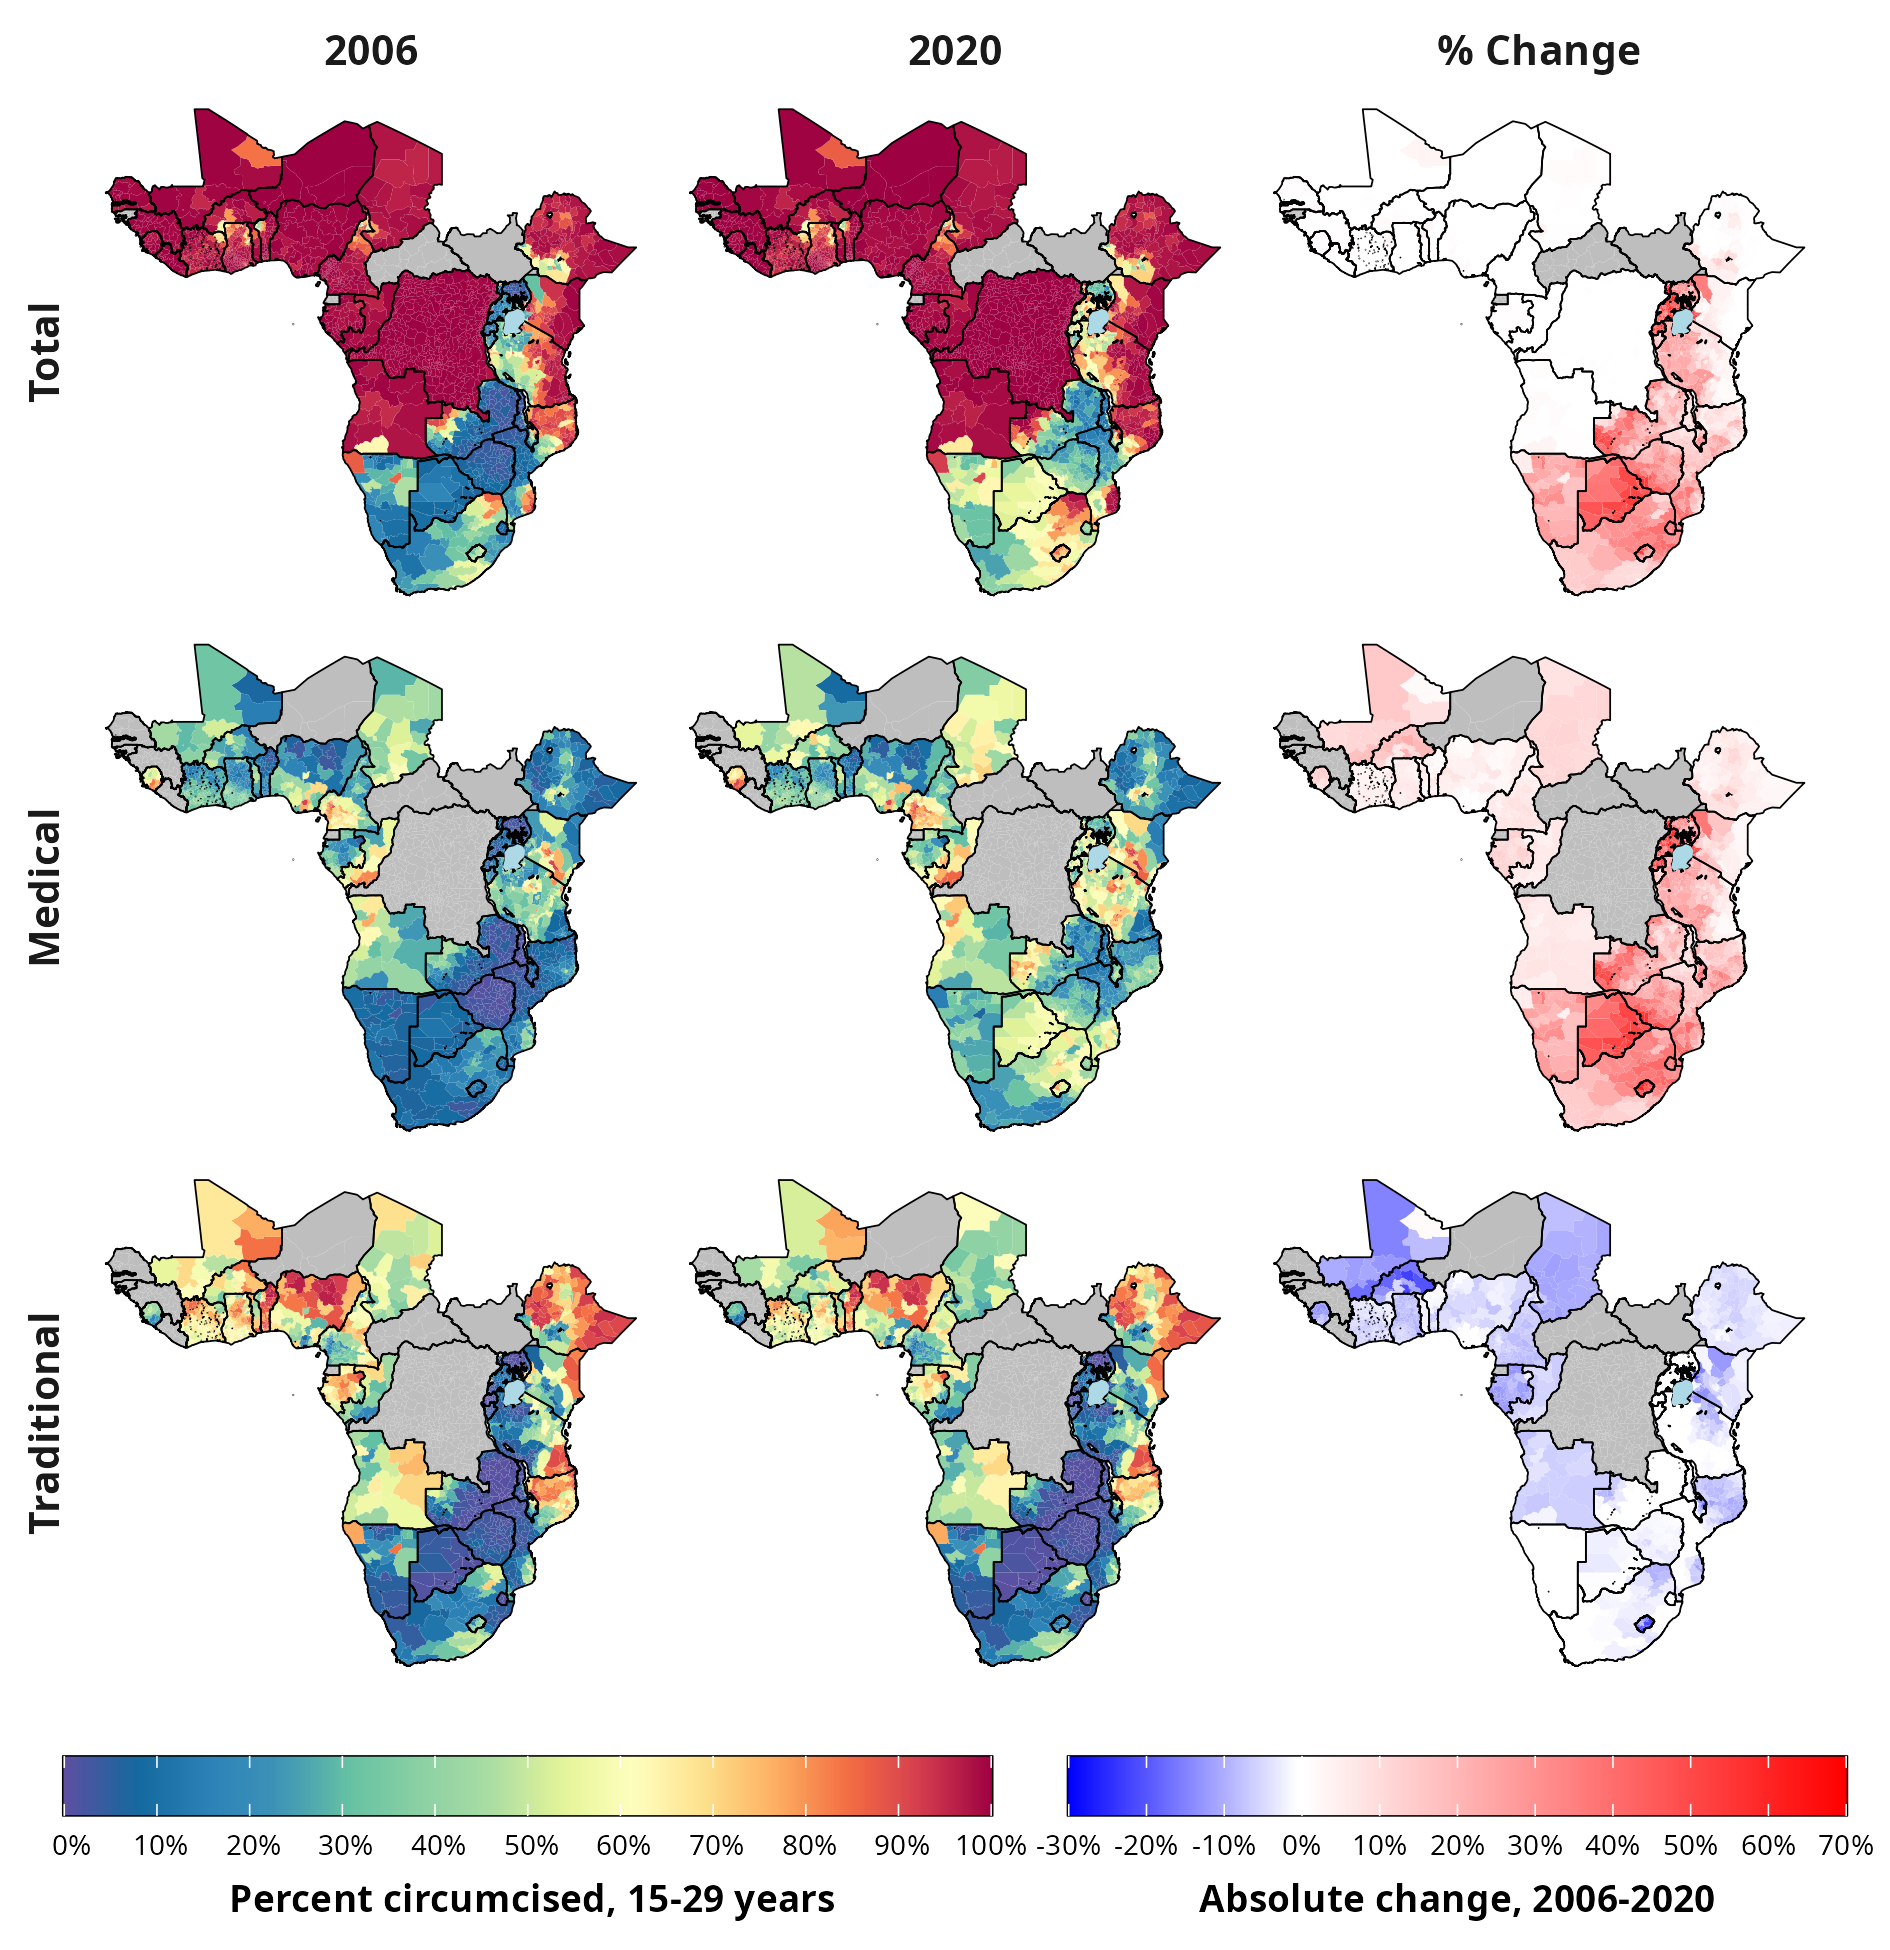
\includegraphics[width=1\linewidth]
    {figures/paper/01_map_plot_facet.png}
    \caption{\emph{Estimated percentage of men aged 15-29 years who were circumcised sub-nationally in 33 sub-Saharan African countries in 2006 and 2020, as well as the difference in coverage between the two years. Maps show total male circumcision (MC), medical male circumcision (MMC) and traditional male circumcision (TMC), respectively. Countries with no information on circumcision type are grey in the Medical and Traditional figures/paper, while countries with no circumcision estimate are grey in all.}}
\end{figure}

% Between 2007, the year VMMC programme implementation began, and 2020, an estimated x million men(95\% CI: x-x million) were newly circumcised. 
% Of these, x million (x-x million) were MMCS, along with x million (x-x million) TMCS. 
% This translated to an increase in MC for the SSA region of x\% (x\%-x\%) in 2010 to x\% (x\%-x\%) in  2020. 
% MC in 2020 ranged from x\% (x\%-x\%) in x to x\% (x\%-x\%) in x, while MMC ranged from x\% (x\%-x\%) in x to x\% (x\%-x\%) in x and TMC ranged from x\% (x\%-x\%) in x to x\% (x\%-x\%) in x. 
% The largest percentage increase in MC coverage from 2010 to 2020 was x\% (x\%-x\%) in x, from x\% (x\%-x\%) to x (x\%-x\%), while for MMC it was x\% (x\%-x\%) in x. 
% The number of annual MCs performed increased from x (x to x) in 2006 to x (x to x) in 2020, a growth of x (x to x) annually. 
% Amongst these, x (x to x) were MMCs in 2006, while in 2020 x (x to x) MMCs were performed, representing an increase in x (x to x) in MMCs performed annually. 
% TMC did not increase anywhere,  and actually decreased in several countries from 2010 to 2020. 
% This is the focus of a later section of our results. 
In 2006, the year before VMMC programme implementation began, an estimated 217.236 million men (95\%
CI: 211.079-222.008 million) were circumcised in the 33 countries in SSA for which we have valid circumcision
data. 
Of these, 67.021 million (62.554-73.259 million) were MMCS, and 102.286 million (95.718-106.665
million) were TMCS. 
This contrasts with 2020, where an estimated 337.913 million males (316.265-362.898
million) were circumcised in these same countries, of which 125.738 million (106.081-157.406 million) were
performed as MMCS, and 136.555 million (124.189-144.146 million) as TMCS. 
\todo{I believe this value is cumulative, not for each discrete year! May need to reword}
% \todo{Can use n_circs_fun function for this\!}
This constituted an increase
of 120.677 million (105.185-140.89 million) newly circumcised males between 2006 and 2020, with 58.717
million (43.528-84.147 million) new MMCs performed, and 34.269 million (28.471-37.481 million) new
TMCs performed. 
The disparity between the number of MCs performed and the number of MMCs performed
can be explained by recalling that for five countries, Liberia, Senegal, Niger, Guinea and the Democratic
Republic of the Congo, we have no circumcision type information, and so can only estimate MC, not MMC or
TMC. 
This translated to a change in mean MC coverage for the SSA region from 57.62\% (59.13\%-55.55\%
) in 2006 to 63.2\% (66.94\%-59.71\%) in 2020, or an increase of 5.58\% (4.16\%-7.81\%). 
MMC coverage increased from 18.75\% (17.75\%-19.9\%  in 2006 to 26.09\% (23.11\%-30.04\%) in 2020, an increase of 7.33\%
(5.36\%-10.14\%). 
TMC changed from 24.64\% (23.57\%-25.58\%) in 2006 to 22.75\% (21.34\%-24.06\%) in 2020, a decrease of 1.89\% (1.51\%-2.23\%).

MC coverage in each country in 2006 ranged from 4.97\% (4.78\%-5.16\%) in Zimbabwe to 95.99\% (86.43\% -
(99.72\%) in Guinea, while MMC in 2006 ranged from 1.63\% (1.47\%-1.76\%) in Zimbabwe to 60.05\% (56.56\%-64.15\%) in Congo and TMC ranged from 0.93\% (0.75\%-1.12\%) in Eswatini to 65.19\% (63.41\%-6.94\%)
in Benin. In contrast, in 2020 MC coverage was estimated to have ranged from 13.77\% (10.51\%-18.87\%) in
Zimbabwe to 96.95\% (89.74\%-99.91\%) in Senegal, while MMC ranged from 11.55\% (8.24\%-16.68\%) in
Zimbabwe to 64.08\% (61.16\%-67.11\%) in Sierra Leone and TMC ranged from 0.69\% (0.56\%-0.84\%) in
Eswatini to 63.02\% (59.34\%-66.65\%) in Benin.

The largest percentage increase in MC coverage from 2006 to 2020 was in Lesotho at 21.7\% (18.66\%-25.93\%),
from 30.06\% (29.53\%-30.7\%) in 2006 to 51.76\% (48.19\%-56.63\%) in 2020, while the highest percentage
increase in MMC was also in Lesotho at 21.49\% (18.14\%-26.13\%), from 6.37\% (5.93\%-6.88\%) in 2006 to
27.86\% (24.08\%-33.01\%) in 2020. For TMC, the largest percentage decrease between 2006 and 2020 was in
Ghana at 8.76\% (6.09\%-9.61\%), from 58.2\% (55.2\%-60.8\%) in 2006 to 49.44\% (45.58\%-54.71\%) in 2020.

The number of annual MCs performed increased from 0.29 million (0.23-0.38 million) in 2006 to 0.29 million
(0.23-0.38 million) in 2020, a growth of 0.1 million (0.056-0.127 million) annually, averaged across all
interceding years. Amongst these, 0.29 million (0.23-0.38 million) were MMCs in 2006, while in 2020 0.391
million (0.287-0.506 million) MMCs were performed, representing an increase in million (0.012-0.166
million) in MMCs performed annually. The number of TMCs performed annually did increase slightly from
2006, from 0.12 million (0.115-0.125 million) to 0.128 million (0.085-0.159 million) in 2020. However,
TMC coverage actually decreased in many countries from 2006 to 2020. This is the focus of section \ref{sec:org5fb5e18}.

% Subnational coverage plot
\begin{figure}[H]
    \centering
    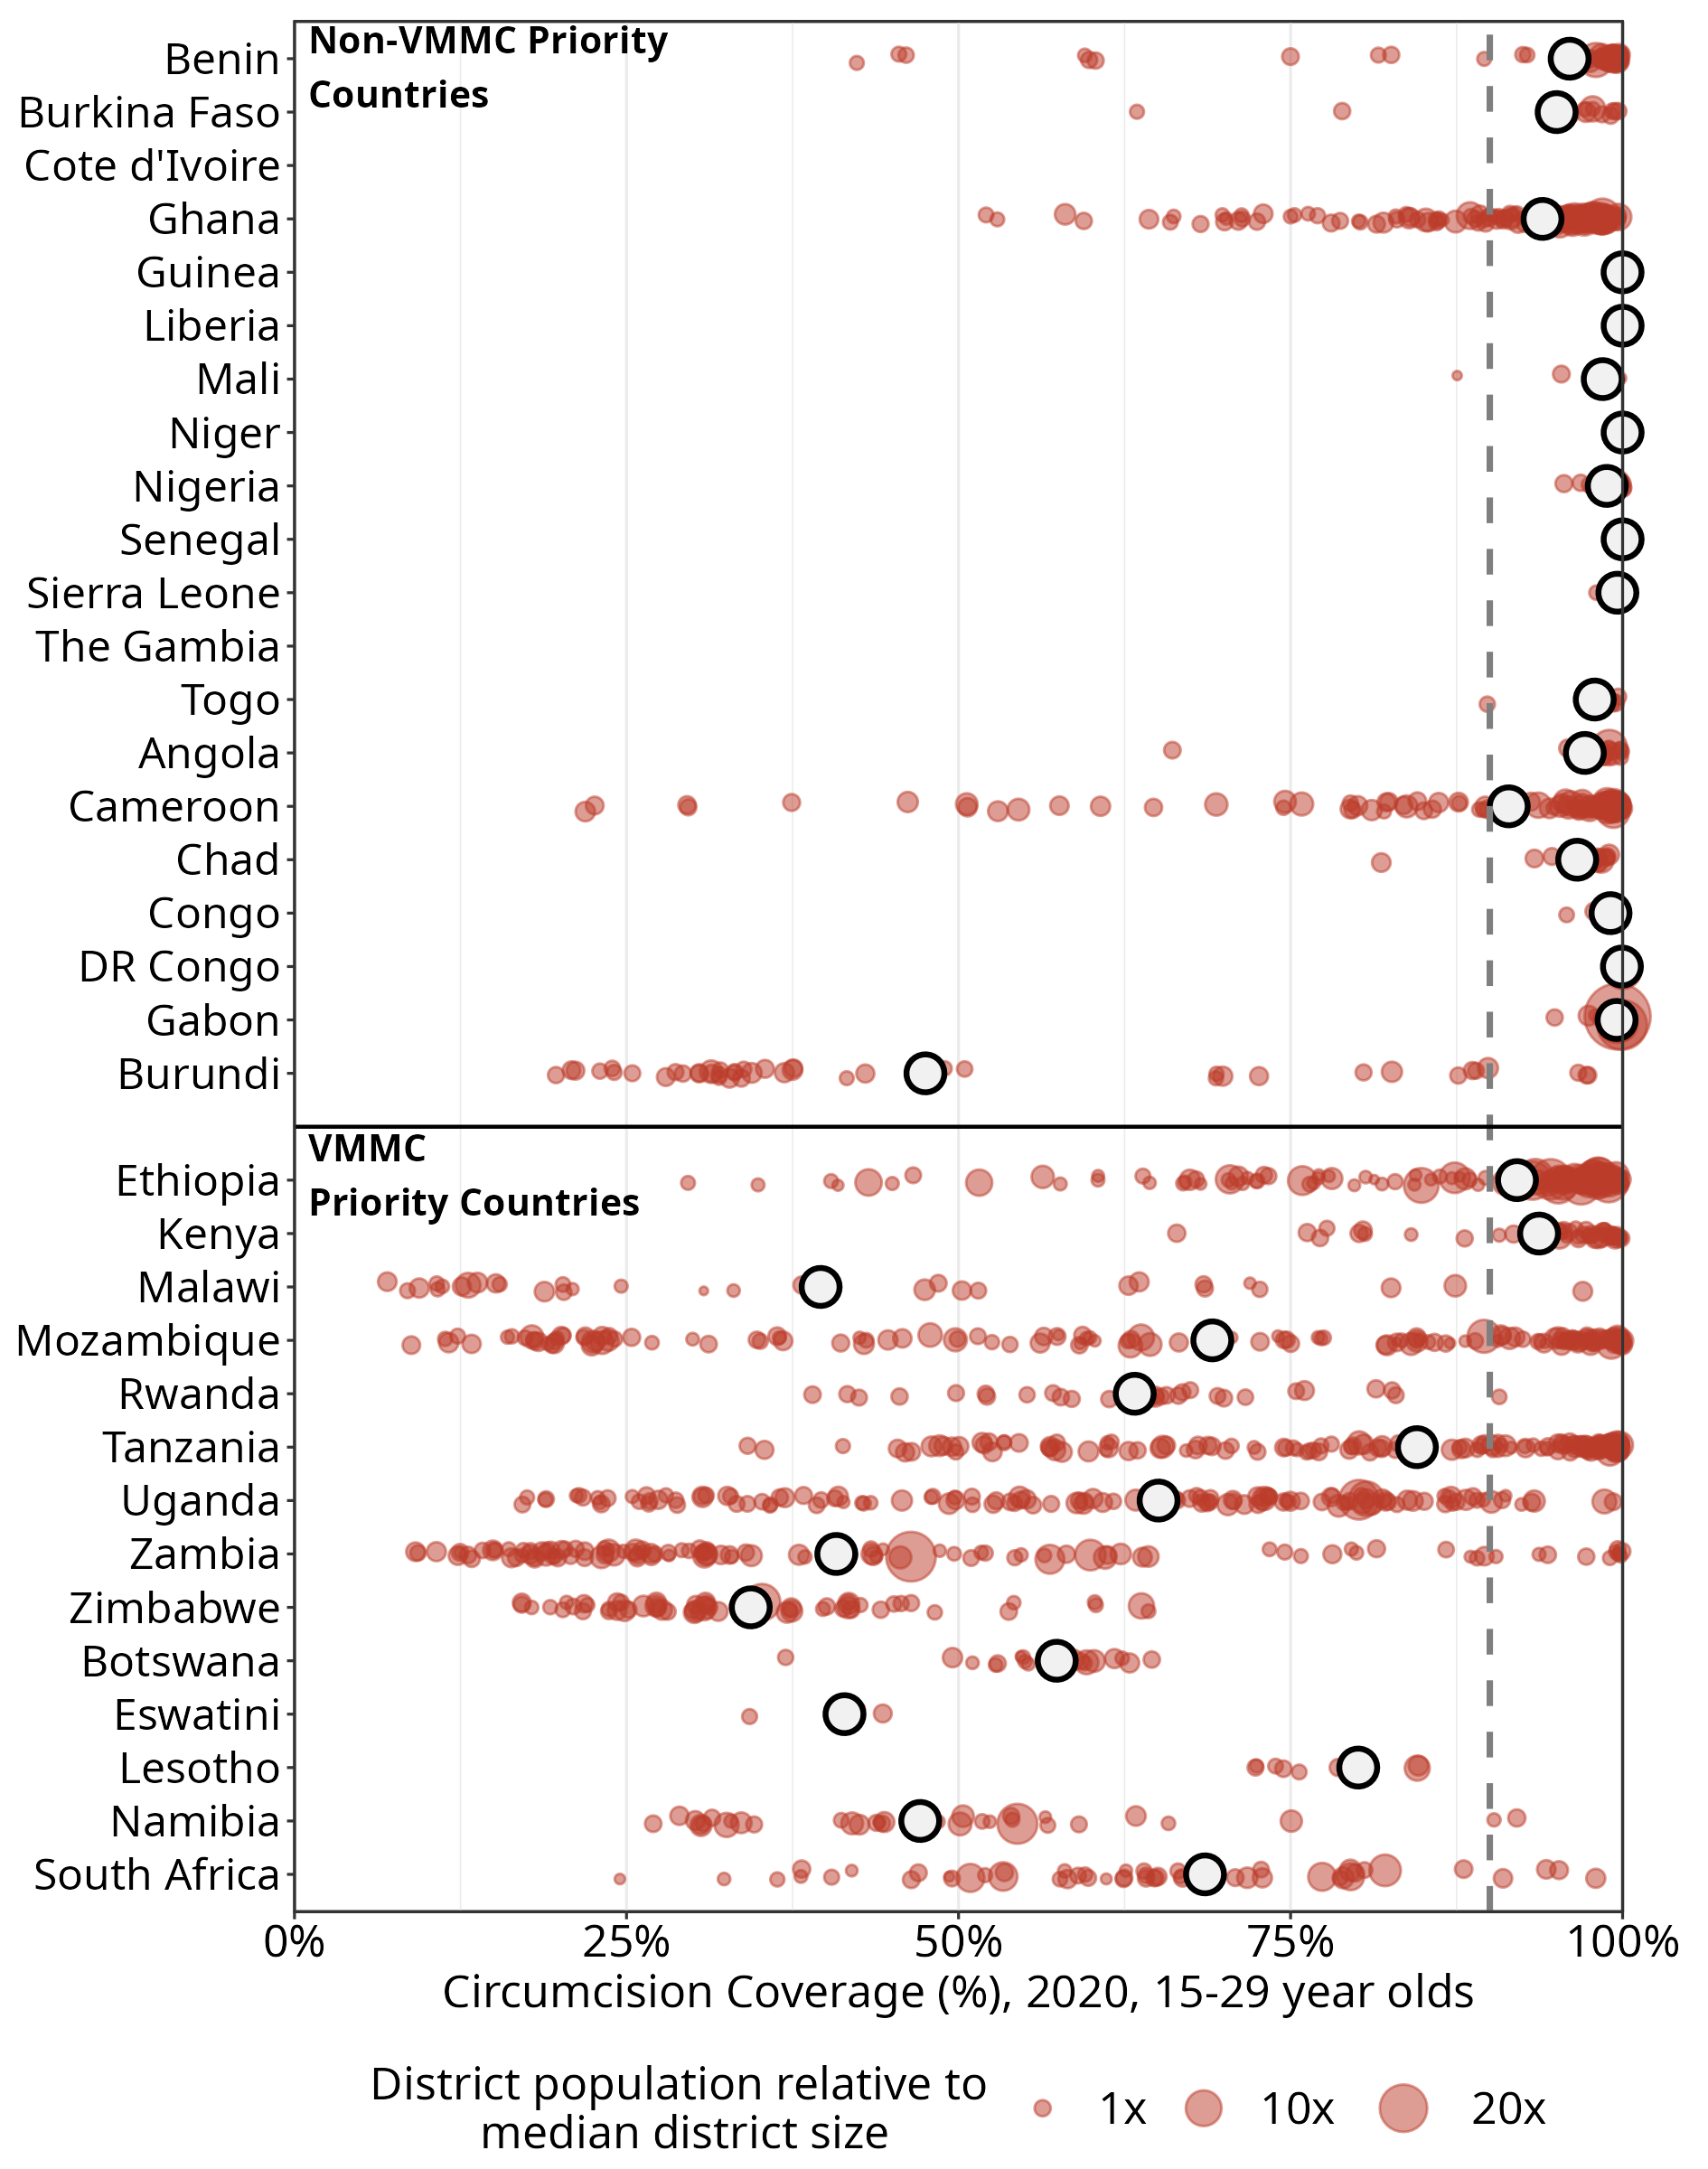
\includegraphics[width=.9\linewidth]
    {figures/paper/02_subnat_plot.png}
    \caption{\emph{District-level median percentage of men aged 15-29 years who were circumcised in 2020 in 33 SSA countries.
    Each point is a district, sized by district population relative to average district size.
    Each white dot represents the national median. 
    A vertical dotted line signifies the UNAIDS target of 90\% national male circumcision amongst 15-29 year olds. The countries below the horizontal black line are VMMC priority countries. VMMC = Voluntary Medical Male Circumcision.}}
\end{figure}

Within countries, the median difference in MC coverage between districts with lowest and highest coverage in 2020 was 56.01\% The smallest variation was in Lesotho, at 48.97\% in Qacha’s Nek to 55.26\% in Berea, while the largest variation was in Mozambique, at 5.35\% in Chifunde to 77.9\% in Homoíne. 
The median difference within countries in MMC coverage between districts with lowest and highest coverage in 2020 was 38.69\% The smallest variation was in Eswatini, at 16.94\% \% in Shiselweni to 24.69\% \% in Manzini, while the largest variation was in Tanzania, at 7.81\% \% in Tandahimba DC to 74.87\% \% in Iringa MC. 
For TMC coverage, the median difference between districts in 2020 was 55.54\% The smallest variation was in Eswatini, at 0.97\% in Eenhana to 79.51\% in Okakarara, while the largest variation was in Namibia, at 0.45\% in Lubombo to 100\% in Manzin. 

\todo{Include comparisons of VMMC vs non-VMMC priority countries, as in below sections}
\todo{Include more commments on results, as below}

\todo{
-Check UNAIDS target for 15-29 year olds, may be 80\%? May want to remove this line altogether?
}

% Within countries, the median difference in MC coverage between the districts with lowest and highest coverage in 2020 was x\% (x\%-x\%).
% For ESA countries, this was x\% (x\%-x\%), in contrast to WCA countries, where it was x\% (x\%-x\%).
% The largest variation overall (and ESA) was in x, from x\% in x to x\% in x, while the largest variation for WCA countries was x, from x\% in x to x\% in x. 
% In total, the mean percentage of districts in each country with greater than 90\% MC coverage amongst those aged 10-29 was x\%. In ESA, this was x\%, while in WCA, this was x\%. 


\subsection{Subnational variation in total, medical \& traditional circumcision across different ages}

% Geofaceted plot of 2020 coverage by age
\begin{figure}[H]
    \centering
    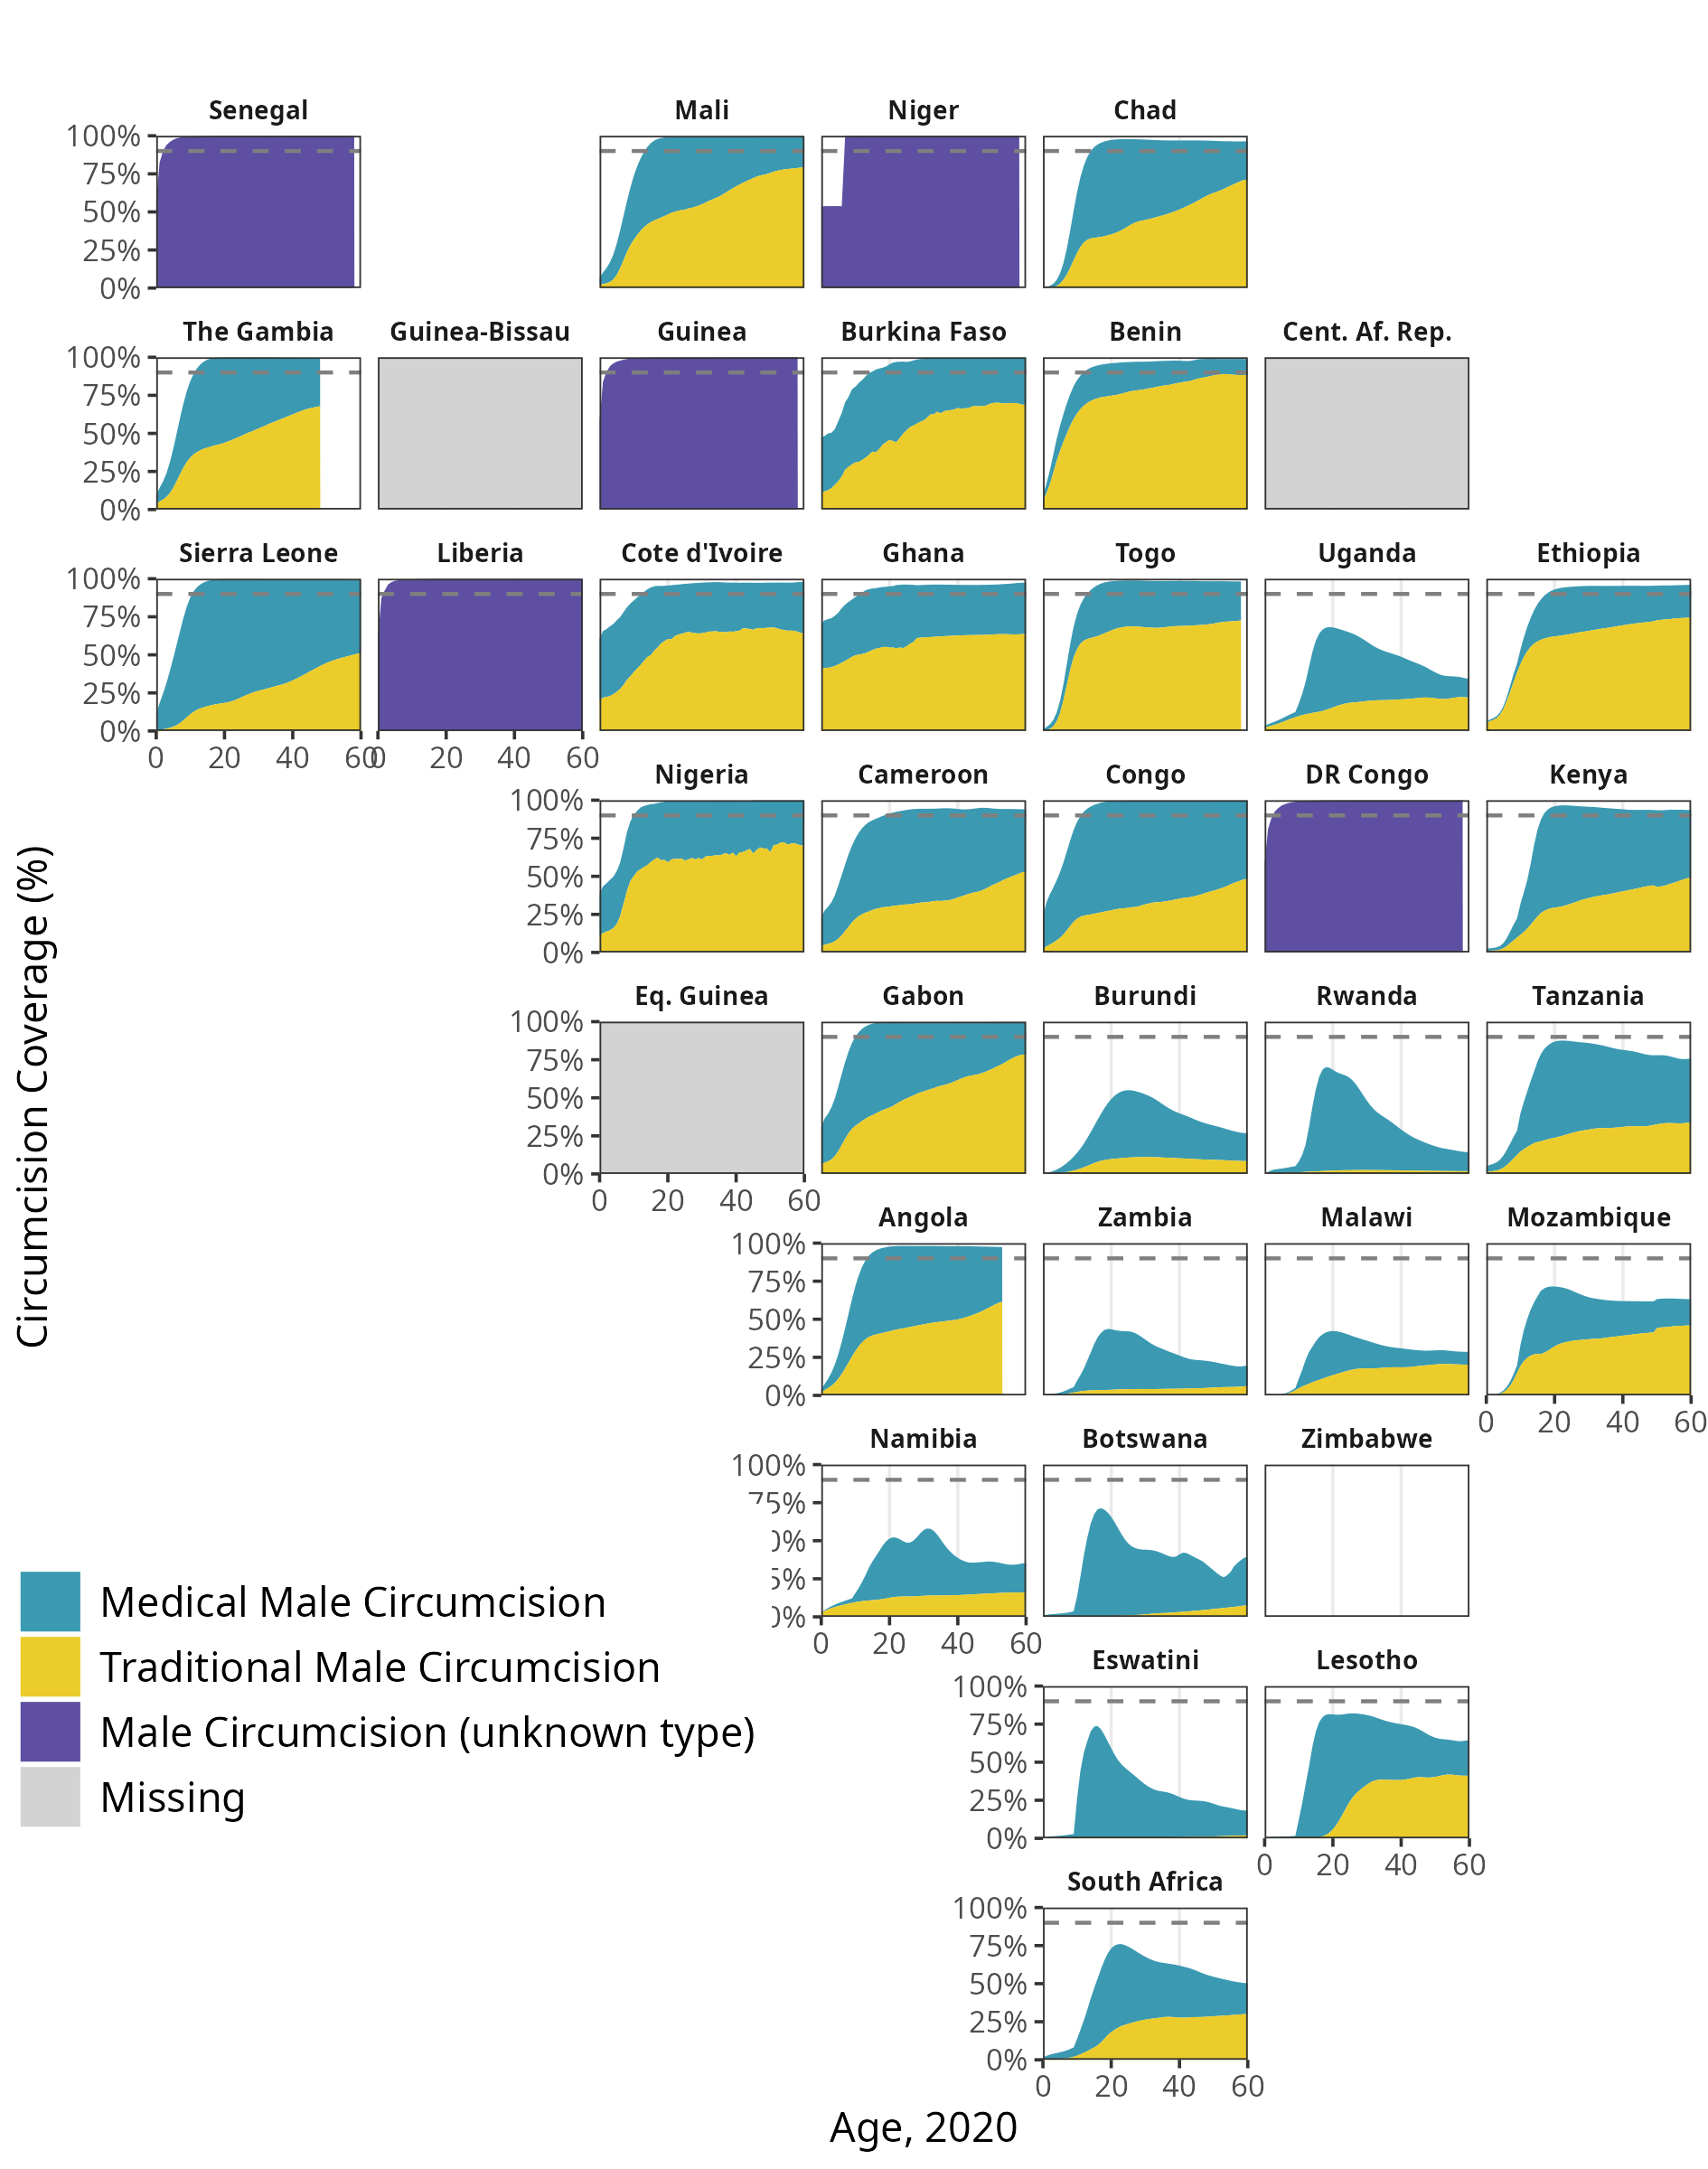
\includegraphics[width=.9\linewidth]
    {figures/paper/03_geo_age.png}
    \caption{\emph{Projected percentage of men from 0 to 60 years old who were medically circumcised and traditionally circumcised by 2020. The horizontal grey dashed line indicates the 90\% circumcision coverage by 2021 target established by the UNAIDS Fast Track strategy. Purple areas represent countries where circumcision type could not be ascertained from surveys, and so shows total male circumcision. Cent. Af. Rep. = Central African Republic, Eq. Guinea = Equatorial Guinea.}}
\end{figure}

Age at circumcision differed greatly by circumcision type and location. The five-year age group in 2006, the year before VMMC programme implementation began, which had the highest MC coverage across the SSA region was 25-29, at 74.1\% (73.13\%-74.73\%). 
In contrast, the age group with the highest MC coverage in 2020 was 20-24, at 84.04\% (82.23\%-86.18\%). The five-year age group in 2006 which had the highest MMC coverage was 20-24, at 25.33\% (23.84\%-26.87\%). 
The age group with the highest MMC coverage in 2020 was also 20-24, at 40.28\% (37.29\%-43.71\%). The five-year age group in 2006 which had the highest
TMC coverage was 45-49, at 40.29\% (36.7\%-43.09\%). The age group with the highest TMC coverage in
2020 was 54-59, 38.55\% (36.19\%-40.5\%). This decrease in the five-year age group with the highest MC coverage, increase in the age group for TMC with the highest coverage (as well as a decrease in coverage for
the highest five-year age group), and increase in overall MMC coverage across the SSA region is indicative of
the effect of VMMC programme implementation on the region.

We may compare changes in circumcision amongst two age groups; 15-29 year olds, which are a particular focus for VMMC implementation, and 30-49 year olds, which are not. MC coverage amongst 15-29 year olds increased from 71.91\% (70.81\%-72.47\%) in 2006 to 82.44\% (80.19\%-85.11\%) in 2020. In contrast, MC
coverage amongst 30-49 year olds only increased from 73.62\% (72.66\%-74.39\%) in 2006 to 78.84\% (77.97\%
- 79.91\%) in 2020. Therefore, MC coverage across SSA saw greater increases in this younger age group
than in this older one, in line with VMMC programme age focus. Similarly, MMC coverage amongst 15-29
year olds increased from 24.84\% (23.49\%-26.22\%) in 2006 to 39.05\% (35.63\%-43.08\%) in 2020, while
MMC coverage amongst 30-49 year olds increased from 22.74\% (21\%-24.74\%) in 2006 to 31.25\% (29.4\% -
33.38\%) in 2020. Therefore, MMC coverage across SSA also saw greater increases amongst 15-29 year olds
than amongst 30-49 year olds. The changes seen in TMC, however, contrast to these larger increases in MC
and MMC coverage for 15-29 year olds. TMC coverage amongst 15-29 year olds decreased from 32.01\% (
30.68\%-33.33\%) in 2006 to 28.25\% (26.57\%-29.88\%) in 2020, while TMC coverage amongst 30-49 year
olds decreased from 38.42\% (36.58\%-40.09\%) in 2006 to 35.1\% (33.64\%-36.58\%) in 2020. Thus, TMC
coverage decreased less in absolute terms amongst 30-49 year olds than amongst 15-29 year olds, which is line
with the greater focus on performing MMCs amongst this younger age group.

Finally, we can contrast patterns in circumcision pattern for different age groups amongst VMMC and
non-VMMC priority countries, where differences in 2006 and 2020 levels and patterns of circumcision seem to
be more pronounced.
For VMMC priority countries, five-year age group MC coverage 2006 was highest amongst 35-39 year olds, at
44.21\% (43.31\%-45.14\%), but in 2020 was highest amongst 20-24 year olds, at 66.08\% (62.71\%-70.35\%
), respectively. This highlights both the increased prevalence of MC in VMMC priority countries, and the
downward shift in age profile of those who are circumcised, since VMMC programme implementation began.
In 2006 MMC coverage was highest amongst 30-34 year olds, at 18.48\% (17.48\%-19.52\%). This contrasts
with 2020, where MMC coverage was highest amongst 20-24 year olds, at 46.71\% (x 43.1\%-x 51.26\%).
This shows that much of the downward shift in age profile of circumcised individuals since 2006 has been
“driven” by an increase in the number of MMCs performed amongst younger individuals. In 2006, TMC
coverage was greatest in 54-59 year olds, at 27.82\% (26.6\%-29.09\%). while in 2020 it was most prevalent
in 54-59 year olds, at 27.82\% (26.6\%-29.09\%, highlighting that VMMC implementation has been focused on areas where TMC has not historically been widely prevalent, and so seems to have had little effect on patterns of TMC in VMMC priority countries, both in terms of its age profile and prevalence.

We can contrast this with the non-VMMC priority countries in SSA. The five-year age group MC coverage in
both 2006 and 2020 was highest amongst 25-29 year olds, at 94.72\% (93.64\%-95.25\%) and 96.15\% (95.67\%
- 96.59\%), respectively. This indicates that MC has increased slightly in non-VMMC priority countries,
but the age profile (in terms of the five-year age group with the highest coverage) has not noticeably changed.
However, in 2006 MMC coverage was highest amongst 15-19 year olds, at 31.13\% (29.27\%-33.01\%). This
contrasts with 2020, where MMC coverage was highest amongst 20-24 year olds, at 36.11\% (x 33.52\%-38.81\%), showing an interesting shift upwards in age for MMCs in non-VMMC priority countries, as a result
of VMMC focus on young adults, as well as a general increase in MMC coverage in these countries. 
In 2006, TMC coverage was greatest in 45-49 year olds, at 49.27\% (43.79\%-53.39\%). while in 2020 it was most
prevalent in 45-49 year olds, at 49.27\% (43.79\%-53.39\%, highlighting a shift upwards in TMCs in VMMC
priority countries, likely resulting from previously TMCs being performed as TMCs.
Similarly, we can compare the 2006 and 2020 circumcision levels amongst 15-29 and 30-49 year olds in both
VMMC and non-VMMC countries, respectively.

In VMMC priority countries, MC coverage amongst 15-29 year olds increased from 37.96\% (37.34\%-38.59\%
) in 2006 to 63.22\% (58.98\%-68.58\%) in 2020. In contrast, MC coverage in 30-49 year olds went from
43.88\% (43.14\%-44.67\%) in 2006 to 54.52\% (53.04\%-56.52\%) in 2020. Therefore, MC coverage in VMMC
priority countries increased amongst 15-29 year olds at a higher rate than amongst 30-49 year olds, and
indeed greater than in SSA as a whole, highlighting the effects of VMMC implementation in these countries
since 2006. Similarly, MMC coverage amongst 15-29 year olds increased from 16.18\% (15.5\%-16.89\%) in
2006 to 44.44\% (39.95\%-50.07\%) in 2020, while MMC coverage amongst 30-49 year olds increased from
17.89\% (17.01\%-18.78\%) in 2006 to 29.9\% (28.28\%-32.11\%) in 2020. Therefore, MMC coverage in
VMMC priority countries also saw greater increases amongst 15-29 year olds than amongst 30-49 year olds,
and greater increases than for SSA as a whole. Again, TMC coverage amongst both fifteen year age groups
contrast to these increases for MC and MMC. TMC coverage amongst 15-29 year olds decreased from 21.78\%
(21.15\%-22.37\%) in 2006 to 18.78\% (18.08\%-19.42\%) in 2020, while TMC coverage amongst 30-49 year
olds decreased from 25.99\% (25.24\%-26.74\%) in 2006 to 24.62\% (23.89\%-25.32\%) in 2020. This decrease
in TMC coverage can partly be attributed to a combination of increased population in non-TMC practising
areas, but TMC coverage also decreased less in absolute terms amongst 30-49 year olds than amongst 15-29
year olds, which is line with the greater focus on performing MMCs, and hence replacing TMCs, amongst
this younger age group.

For non-VMMC priority countries, MC coverage in 15-29 year olds increased from 93.98\% (
92.57\%-94.49\%) in 2006 to 94.94\% (93.98\%-95.85\%) in 2020, staying relatively similar. MC coverage in
30-49 year olds also increased from 93.97\% (92.85\%-94.72\%) in 2006 to 95.48\% (95.03\%-95.92\%) in 2020,
so again, when taking our credible intervals into account, there was little increase amongst this age group in
non-VMMC priority countries. It is interesting that MC seems to have increased more amongst 30-49 year
olds than amongst 15-29, defying the trend amongst VMMC priority countries and SSA as a whole. MMC
coverage amongst 15-29 year olds increased from 30.48\% (28.69\%-32.28\%) in 2006 to 35.55\% (32.82\% -
38.54\%) in 2020, while MMC coverage amongst 30-49 year olds increased from 26.06\% (23.72\%-28.81\%) in
2006 to 32.17\% (30.17\%-34.24\%) in 2020. Hence, MMC coverage in non-VMMC countries also saw greater
increases amongst 30-49 year olds than in 15-29 year olds, but not much change overall when factoring in our
uncertainty. TMC coverage amongst 15-29 year olds decreased from 38.67\% (36.88\%-40.45\%) in 2006 to
34.41\% (32.09\%-36.68\%) in 2020, while TMC coverage amongst 30-49 year olds decreased from 46.93\%
(44.34\%-49.23\%) in 2006 to 42.26\% (40.3\%-44.29\%) in 2020. Thus, TMC coverage decreased less in
absolute terms amongst 30-49 year olds than amongst 15-29 year olds, which is line with the greater focus on
performing MMCs amongst this younger age group. TMC coverage decreased more amongst non-VMMC
countries for both age groups, suggesting likely replacement of historical TMC with MMC.

\subsection{Subnational heterogeneity in age at medical and traditional circumcision}

% Geofaceted plot of 2020 coverage by age
\begin{figure}[H]
    \centering
    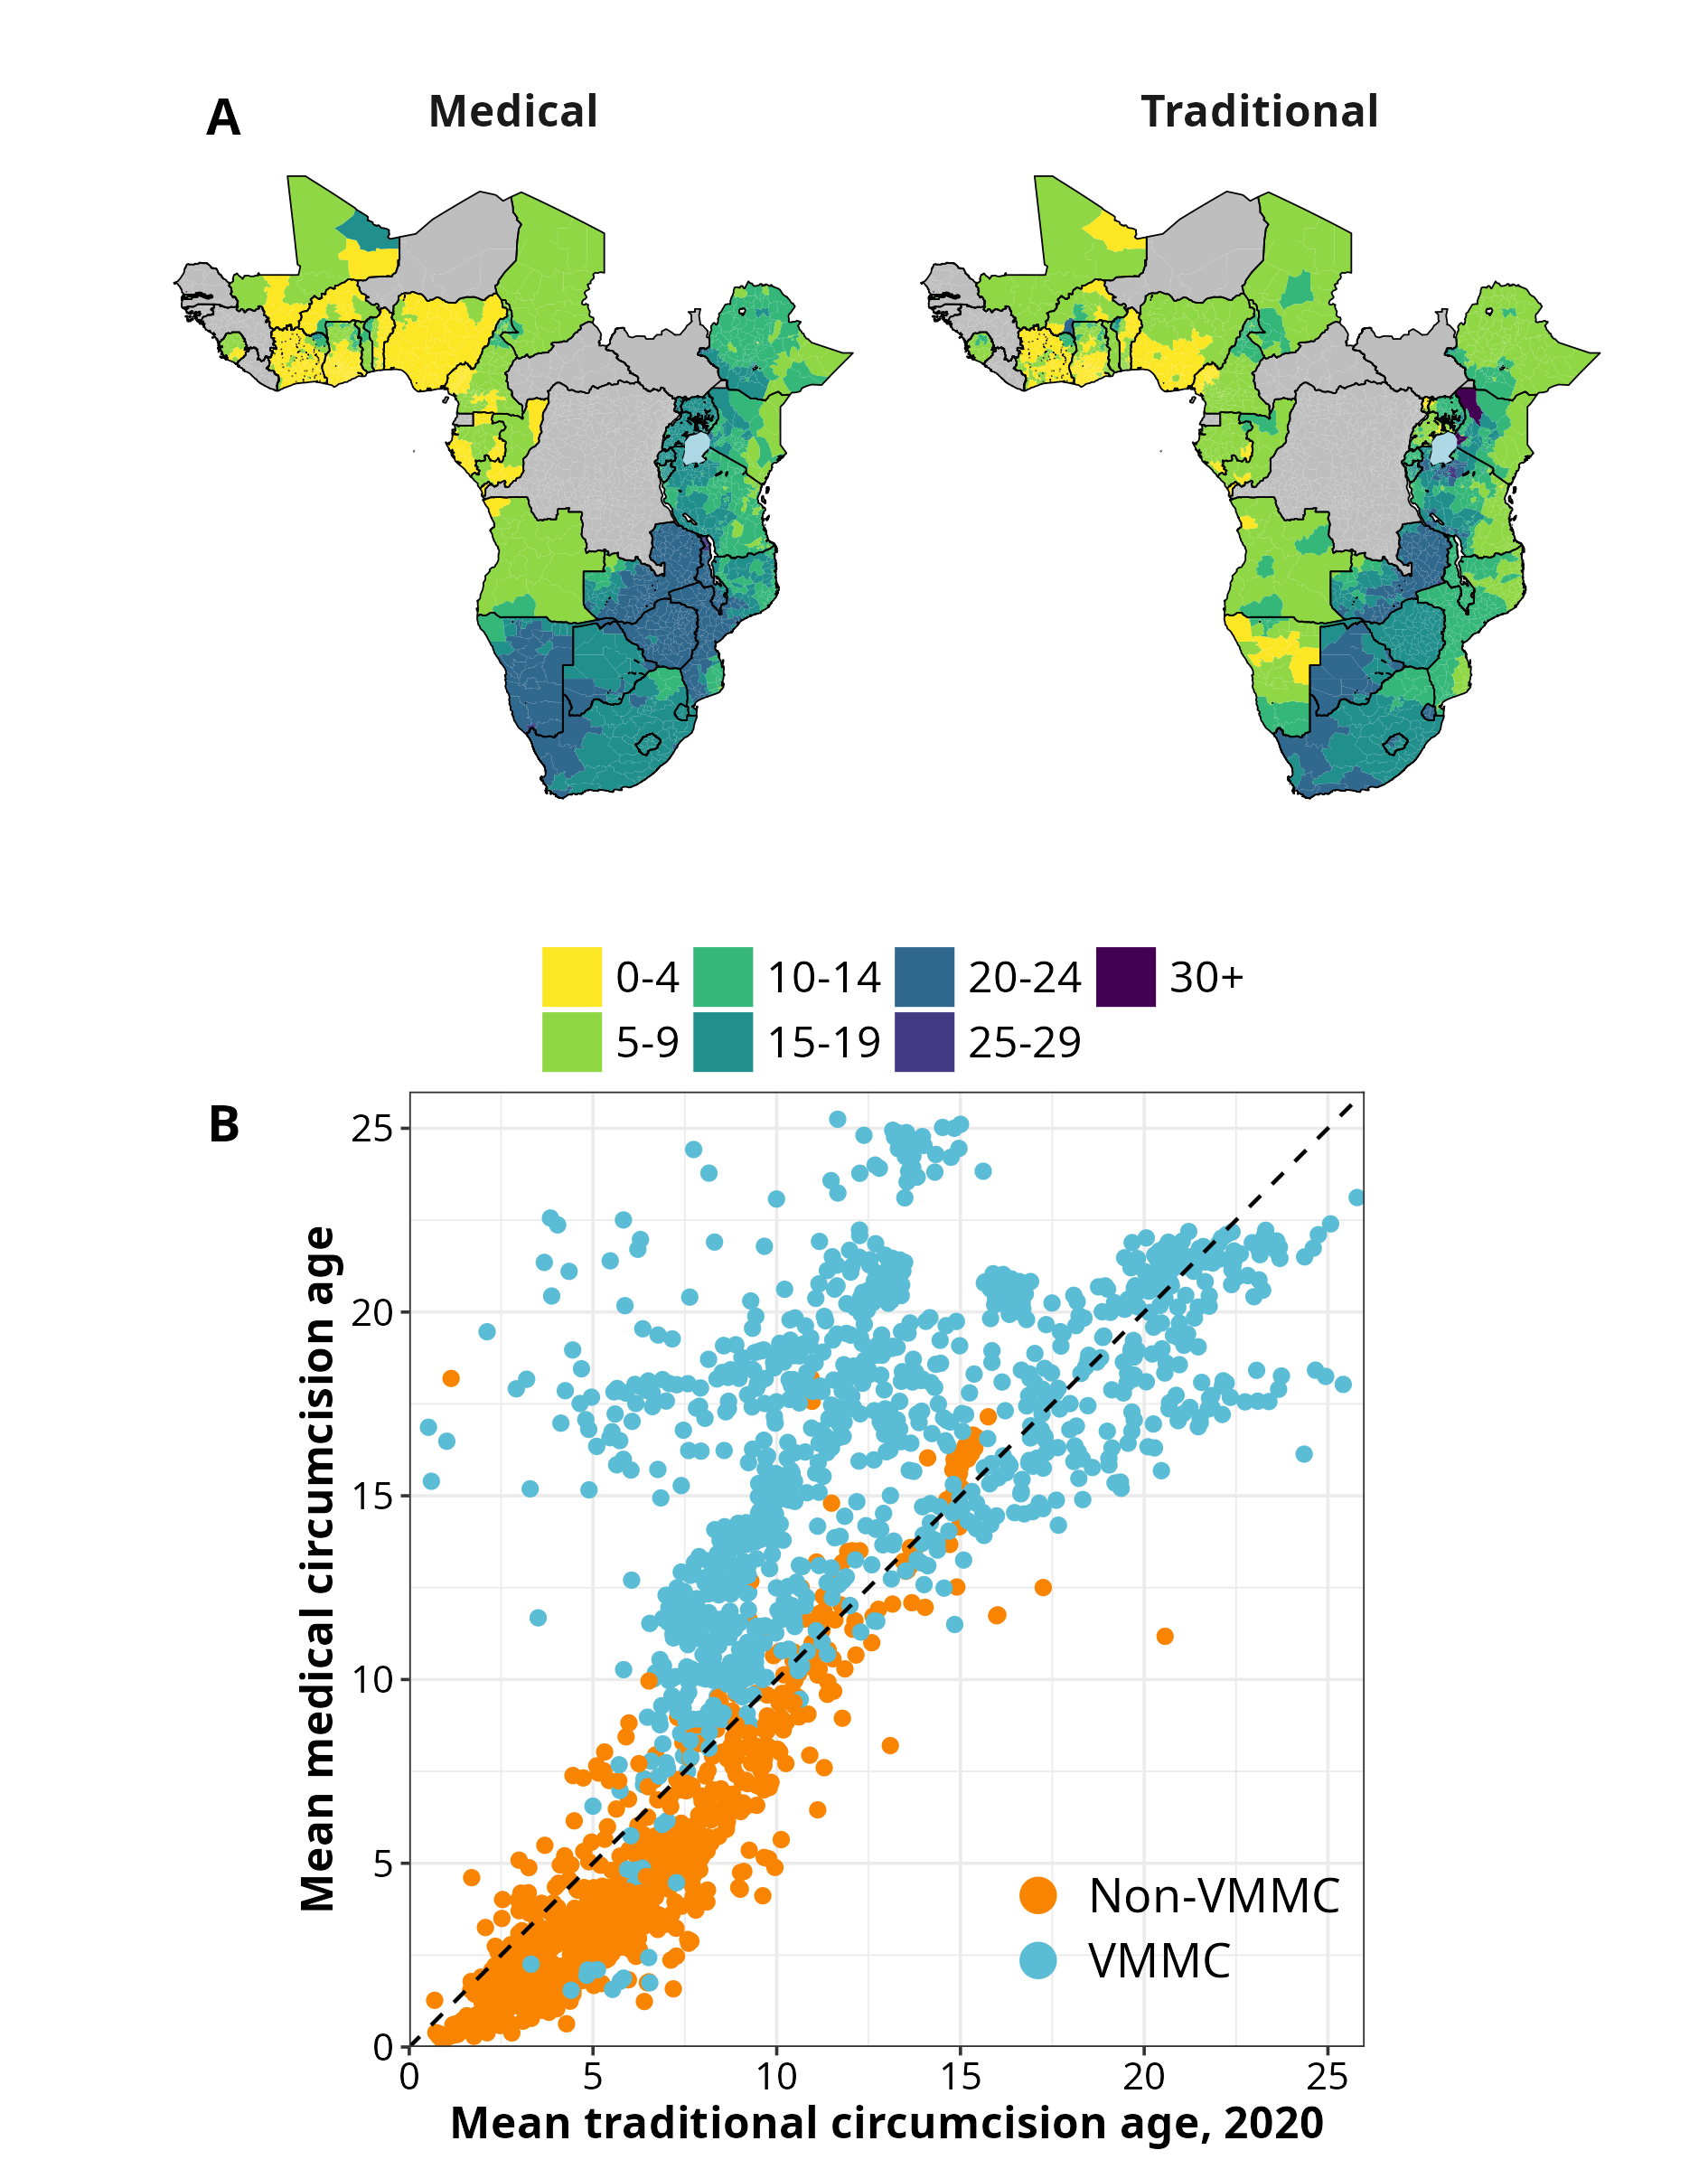
\includegraphics[width=.9\linewidth]
    {figures/paper/04_map_plot_mean_circ_age.png}
    \caption{\emph{(A) Estimated distinct-level age at circumcision in 2020 in 33 sub-Saharan African countries. Maps show mean medical male circumcision (MMC) and mean traditional male circumcision (TMC) age. Countries without estimates are in grey. Mean circumcision ages are binned into five-year age groups and over 30s. (B) Scatterplot of district-level mean traditional male circumcision age versus mean medical male circumcision age. A diagonal dashed line passes through the origin and (25, 25). Points representing each district are coloured by whether their country is a Voluntary Male Medical Circumcision (VMMC) priority country.}}
\end{figure}

The mean age at circumcision for MC in 2006 was 8.88 (8.53-9.62), while in 2020 it was 9.26 (8.76-9.78
). Similarly, the mean age at circumcision for MMC in 2006 was 10.59 (10.19-11.38), and in 2020 it was
10.8 (10.35-11.24). Finally, the mean age at circumcision in 2006 for TMC was 9.66 (9.36-10.32), and in
2020 it was 9.35 (8.64-10.08). 
Therefore, the mean age at circumcision for MC and MMC went up slightly from
2006 to 2020. However, it is important to note that the uncertainty ranges in our credible intervals overlap,
so this increase could be seen as “non-significant”, in some sense. In contrast, the mean age at circumcision
for TMC was seen to decrease, altough again, not in a manor that exceeds our uncertainty bounds. This may
suggest that VMMC implementation amongst 15-29 year olds has corresponded to an upward shift of mean
age at circumcision for MC and MMC, and replaced some circumcisions which would previously have been
performed as TMCs, which may explain the observed decrease in mean age of TMC.

As in the previous section, we can also compare how the mean age of circumcision differs amongst VMMC
priority countries, versus their non-VMMC prority counterparts in SSA.

For VMMC priority countries, the mean age at circumcision for MC in 2006 was 14.05 (13.57-14.68), while
in 2020 it was 15.45 (14.24-16.36). Similarly, for MMC in 2006 the mean age at circumcision was 15.82 (
15.24-16.48), while in 2020 it was 16.41 (15.43-17.13). Lastly, the mean age at circumcision in 2006 for
TMC was 12.29 (11.88-13.04), and in 2020 it was 11.46 (10.84-12.43. So the mean age at circumcision for
all circumcision types is higher in VMMC priority countries than overall in SSA, highlighting the historically
low levels of MC and TMC in these countries. Like in SSA overall, the mean age at circumcision for MC and
MMC went up slightly, albeit not significantly when factoring in uncertainty bounds. Again, mean age at
TMC also decreased in VMMC priority countries.

For non-VMMC priority countries, the mean age at MC in 2006 was 5.51 (5.08-6.33), while in 2020 it was
5.24 (5.01-5.5). Similarly, the mean age at MMC in 2006 was 6.07 (5.82-6.95), and in 2020 it was 5.93 (
5.94-6.13). Finally, the mean age at TMC in 2006 for TMC was 7.38 (7.18-7.96), and in 2020 it was 7.52
(6.73-8.06. In contrast to our VMMC priority countries, these countries have a lower mean at circumcision
for all circumcision types, largely driven by high TMC levels historically. It is interesting that the age at
circumcision for MC and MMC actually increased for non-VMMC priority countries, in contrast to SSA as a
whole and the priority countries. Likewise, the mean age at TMC increased. This can be explained
by a possible replacement of TMC with MMC in a traditional setting, so at generally younger ages than
MMCs performed as part of VMMC programmes. This caused a natural shift upwards of the mean age at
TMC, as younger individuals are now more likely to receive MMCs.

% estimated percentage of men aged 15-29 years who were circumcised sub-nationally in 33 sub-Saharan African countries in 2006 and 2020, as well as the difference in coverage between the two years. Maps show total male circumcision (MC), medical male circumcision (MMC) and traditional male circumcision (TMC), respectively. Countries with no information on circumcision type are grey in the Medical and Traditional figures/paper, while countries with no circumcision estimate are grey in all

\subsection{Decrease in traditional male circumcision in sub-Saharan Africa over time}
\label{sec:org5fb5e18}

% Dumbbell of type-specific cov change 00'-20'
% todo: Rewrite caption
\begin{figure}[H]
    \centering
    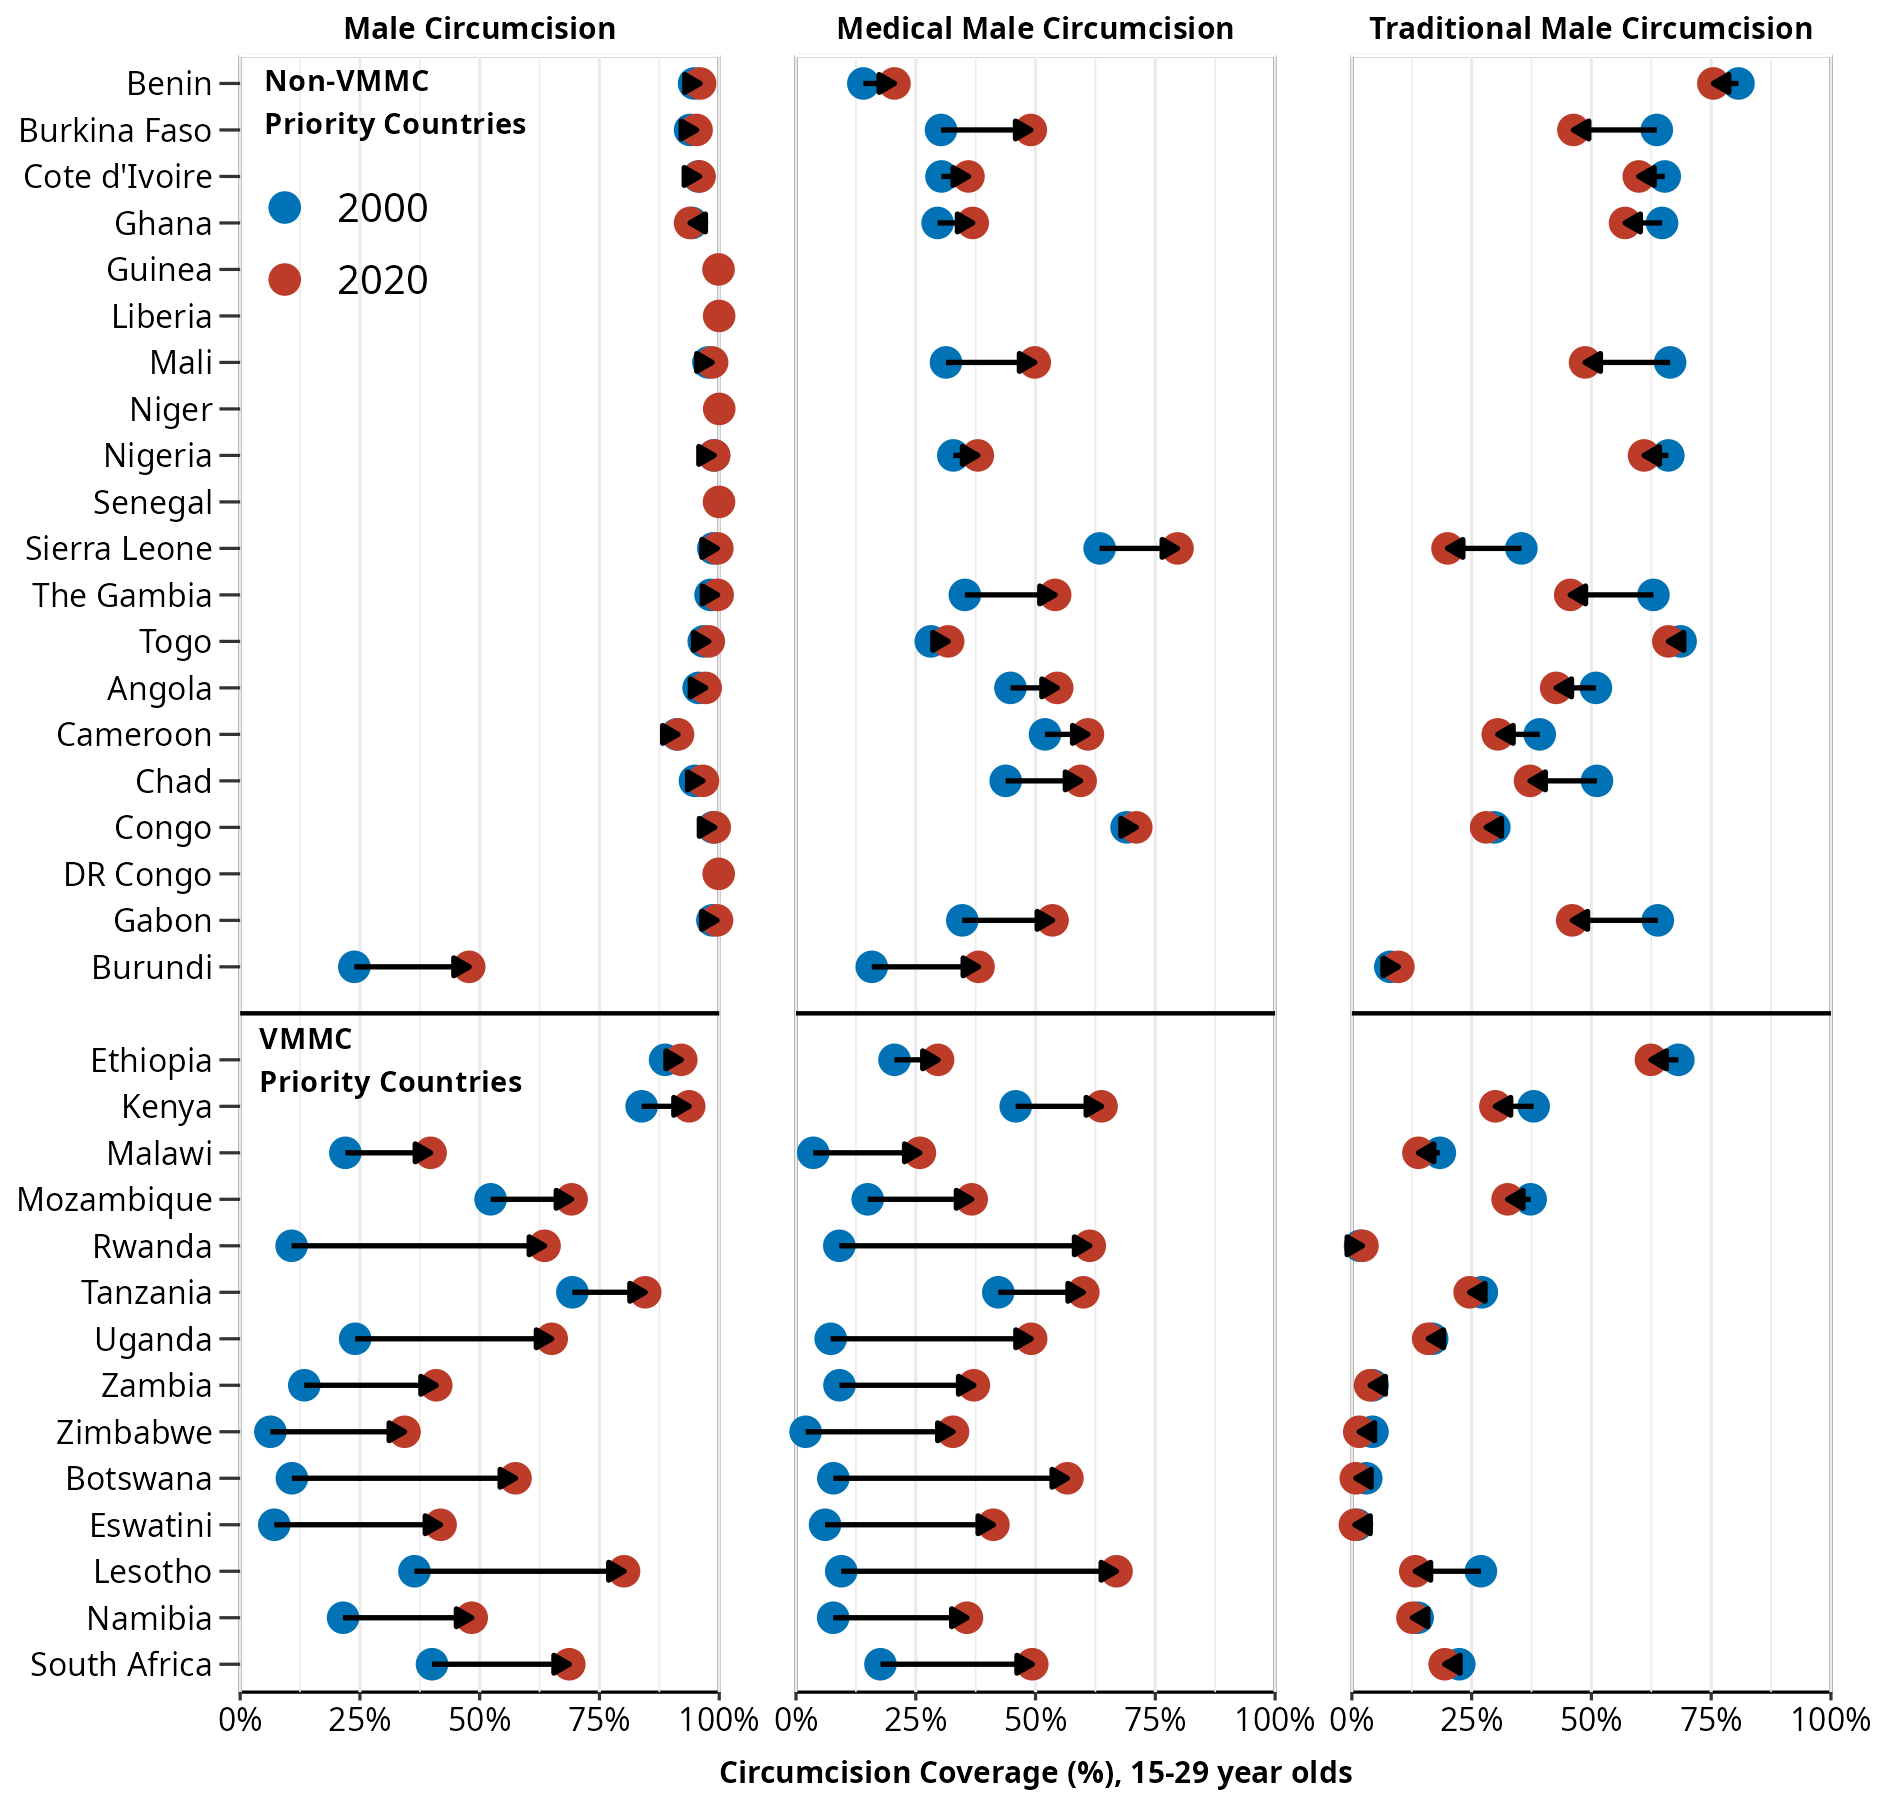
\includegraphics[width=1\linewidth]
    {figures/paper/05_change_00_20.png}
    % \caption{\emph{Absolute difference, in percentage coverage from 2000 to 2020, coloured by sub-Saharan African region. figures/paper are split by circumcision type. Countries are ordered from north to south, east to west, and the 13 countries below the black horizontal lines are VMMC priority countries.  }}
    \caption{\emph{Circumcision coverage in 2000 and 2020 amongst 15-29 year olds in all 34 sub-Saharan African countries, split by circumcision type. The countries below the horizontal black line are VMMC priority countries.}}
\end{figure}

The average TMC coverage in SSA in 2006 was 24.3\% (23.19\% to 25.27\%). This fell to 21.88\% (20.35\% to 23.33\%) in 2020, a decrease of 2.42\%. In non-VMMC priority countries, TMC coverage was 31.26\% (29.71\% to 32.59\%). This fell to 27.66\% (25.4\% to 29.8\%) in 2020, representing a decrease of 3.59\%. In contrast, TMC coverage in VMMC priority countries was 14.36\% (13.88\% to 14.8\%). This fell to 13.63\% (13.13\% to 14.08\%) in 2020, representing a decrease of 0.74\%. Therefore, the decrease in TMC found throughout SSA is much more pronounced for non-VMMC countries.

\todo{Add thousand/million/billion suffix here (or at least commas), rather than whole number!}
In 2006, 98009 (94028-102330) TMCs were performed, while in 2020 this increased to 102827 (63457-129829), representing a 4818 increase in annual TMCs. However, this increase must be taken within the context of a large increase in population in SSA over this period, from 1.23 billion in 2006 to 1.80 billion in 2020, and as seen in our coverage estimates above, constitutes a decrease in the number of TMCs performed per capita in the region (need to calculate this?!) In non-VMMC priority countries, the annual number of TMCs performed changed from 114700 (109648-120604) in 2006 to 117525 (54128-160432) in 2020, or by 2825. This is within the context of the population of non-VMMC priority countries increasing from 749 million to 1.11 billion from 2006 to 2020. In VMMC priority countries, the number of TMCs performed went from 74165 (71715-76224) in 2006 to 74165 (71715-76224) in 2020, a fall of 7665. In VMMC priority countries, the population increased from 481 million to 694 million. \todo{Comment on this}

We can also compare the differences in TMC coverage change between 15-29 and 30-49 year olds, in SSA as a whole and in VMMC and non-VMMC priority countries.

For the 15-29 age group, TMC coverage was reduced from 31.1\% (29.78\% to 32.41\%) in 2006 to 26.69\% (25.05\% to 28.31\%) in 2020, a drop of 4.41\%. This contrasted with the 30-49 age group, where TMC coverage went from 37.45\% (35.52\% to 39.18\%) in 2006 to 34.02\% (32.58\% to 35.48\%) in 2020, a drop of 3.42\%. Therefore, in SSA as a whole TMC coverage decreased slightly more amongst 15-29 year olds than in 30-49 year olds, likely as a result of VMMC programme focus on this age group.

For the 15-29 year olds in non-VMMC priority countries, TMC coverage was reduced from 31.1\% (29.78\% to 32.41\%) in 2006 to 26.69\% (25.05\% to 28.31\%) in 2020, a drop of 4.41\%. This contrasted with the 30-49 age group, where TMC coverage went from 37.45\% (35.52\% to 39.18\%) in 2006 to 34.02\% (32.58\% to 35.48\%) in 2020, a drop of 3.42\%. Therefore in non-VMMC priority countries the decrease in TMC coverage was larger for both age groups than in SSA as a whole, but the difference between this decrease for 15-29 year olds versus 30-49 year olds is less pronounced.

For VMMC priority countries, the 15-29 age group, TMC coverage was reduced from 31.1\% (29.78\% to 32.41\%) in 2006 to 26.69\% (25.05\% to 28.31\%) in 2020, representing a fall of 4.41\%. In the 30-49 age group, TMC coverage in VMMC priority countries dropped from 37.45\% (35.52\% to 39.18\%) in 2006 to 34.02\% (32.58\% to 35.48\%) in 2020, a drop of 3.42\%. Therefore, in VMMC priority countries there is a much greater disparity in the drop in TMC coverage between 15-29 and 30-49 year olds. 15-29 year olds saw a much greater drop in TMC coverage, likely resulting from VMMC programme focus on these ages.

The largest decrease in TMC coverage from 2006 to 2020 was in Côte d’Ivoire, where TMC coverage fell from 58.45\% (57.07\% to 59.5\%) to 48.85\% (46.87\% to 50.49\%, a decrease of 9.6\%.

The largest decrease in TMC coverage amongst VMMC countries was from Côte d’Ivoire, where TMC coverage fell from 58.45\% (57.07\% to 59.5\%) to 48.85\% (46.87\% to 50.49\%, a decrease of 9.6\%.

\todo{add smallest decrease here? Would be more interesting for non-VMMC countries, could show where MMC has not begun to replace TMC}
\todo{add \# of countries in both regions which have experienced a drop in TMC coverage?? Might be interesting for non-VMMC}

\subsection{UNAIDS goals progress amongst 10-29 year olds in Voluntary Male Medical Circumcision target countries}
\label{sec:orgf9204d9}

As a reminder, in 2010 the WHO and UNAIDS set a 80\% MC target for 15-49 year olds in the VMMC
priority countries by 2018. This target was expanded in 2016 to the new target of 90\% MC amongst 10-29
year olds in VMMC priority countries by 2021.
Amongst the 14 VMMC priority countries modelled, 3 countries were projected to have achieved the VMMC
target of 80\% MC coverage amongst 15-49 year olds by 2020, Tanzania, Ethiopia and Kenya. None were
expected to reach the 90\% target for 10-29 year olds. No countries were expected to have reached these goals
in all districts.
MC coverage amongst 10-29 year olds across VMMC priority countries increased from 30.94\% (30.4\% to
31.53\%) in 2006 to 54.09\% (50.78\% to 58.36\%) in 2020, an increase of 23.15\% (20.38\%-26.83\%). MMC
coverage amongst 10-29 year olds across VMMC priority countries increased from 13.68\% (13.07\% to 14.31\%
) in 2006 to 39.24\% (35.76\% to 43.66\%) in 2020, an increase of 25.56\% (22.69\%-29.35\%). MC coverage
amongst 15-49 year olds across VMMC priority countries increased from 38.29\% (37.71\%-38.88\%) in
2006 to 58.7\% (56.58\% to 61.44\%) in 2020, an increase of 20.41\% (18.87\%-22.55\%). MMC coverage
amongst 15-49 year olds across VMMC priority countries increased from 16.87\% (16.22\% to 17.58\%) in
2006 to 39.57\% (37.31\% to 42.48\%) in 2020, an increase of 22.7\% (21.1\%-24.91\%).
Between 2006 and 2020 in these countries, 2.396 million (2.066 million-2.81 million) MCs were performed
on 10-29 year olds. Of these, 2.285 million (2.285 million-2.285 million) were MMCs, and 0.573 million
(0.573 million-0.573 million) were TMCs. Over the same period, million (million-million) MCs were
performed on 15-49 year olds, million (million-million) of which were MMCs, and million (million-million) of which were TMCs.

The number of annual MCs amongst 10-29 year olds increased from 0.702 million (0.648 million to 0.757
million) in 2006 to 1.694 million (1.418 million to 2.053 million) in 2020.
The number of annual MMCs amongst 10-29 increased from 0.431 million (0.383 million to 0.485 million
) in 2006 to 1.441 million (1.16 million to 1.8 million) in 2020, while in constrast, the number of TMCs
decreased from 0.271 million (0.254 million to 0.29 million) in 2006 to 0.252 million (0.222 million to 0.283
million) in 2020.
For 15-49 year olds, the number of annual MCs increased from 0.335 million (0.305 million to 0.367 million)
in 2006 to 0.727 million (0.578 million to 0.919 million) in 2020.
Annual MMCs amongst 15-49 increased from 0.225 million (0.198 million to 0.253 million) in 2006 to 0.648
million (0.498 million to 0.84 million) in 2020, while in constrast, the number of TMCs decreased from 0.11
million (0.101 million to 0.122 million) in 2006 to 0.079 million (0.067 million to 0.092 million) in 2020.
1.694 (1.418 to 2.053) additional circumcisions are required to achieve 90\% and 80\% MC coverage targets
for 10-29 and 15-49 year olds, respectively, across all VMMC priority countries.
This is equivalent to 16.7 (21.3 to 12.6) and 38.3 (38.3 to) times the projected number of MCs for 10-29
and 15-49 year olds for 2020.
MC coverage in 2020 for 10-29 year olds in VMMC priority countries was highest in Ethiopia, at 84.9\% (
82.95\%-87.3\%), and lowest in Zimbabwe, at 29.51\% (27.21\%-32.77\% . For 15-49 year olds, the highest
MC coverage was in Ethiopia, at 84.9\% (82.95\%-87.3\%), and lowest in Zimbabwe, at 29.51\% (27.21\% -
32.77\% . MMC coverage for 10-29 year olds in VMMC priority countries was highest in Lesotho, at 58.11\% (
55.3\%-62.45\%), and lowest in Malawi, at 22.57\% (21.23\%-24.54\% . For 15-49 year olds, the highest MMC
coverage was in Lesotho, at 58.11\% (55.3\%-62.45\%), and lowest in Malawi, at 22.57\% (21.23\%-24.54\% .
The largest increase from 2006 to 2020 in MC coverage for 10-29 year olds amongst VMMC priority countries
was in Botswana, from 9.39\% (8.74\%-10.22\%) in 2006 to 52.52\% (52.52\%-52.52\%) in 2020, a 43.12\% (
40.45\%-44.77\%) increase. In contrast, the lowest increase in MC coverage in these countries was in from
9.39\% (8.74\%-10.22\%) in 2006 to 52.52\% (52.52\%-52.52\%) in 2020, a 43.12\% (40.45\%-44.77\%)
increase.
However, these figures belie significant subnational heterogeneity in MC coverage amongst VMMC priority
countries. 213 (124-301) of 1072 districts in these countries were expected to have reached 90\% MC
coverage amongst 10-29 year olds in 2020, up from 125 (60-203) of 1072 in 2006, before VMMC programmes
began. Similarly, 422 (367-506) of 1072 districts in these countries were expected to have reached 80\% MC
coverage for 15-49 year olds in 2020, compared to 344 (296-392) of 1072 in 2006.
In 2020, 7 (5-8) of the 14 VMMC priority countries had no districts which satisfied the 90\% MC coverage
target for 10-29 year olds. This was down from 10 (8-11) in 2006. Similarly, in 2020, 3 (3-4) countries had no districts which satisfied the 80\% MC coverage target for 15-49 year olds. This was down from 5 (5-5) in 2006.

\todo{Add table here?}

% \subsection{Comparison to results of DMPPT2 model}
% \label{sec:orge0178ca}
% 
% \todo{Write this section!}

\section{Discussion}
\label{sec:orgca35e01}

Sub-national MC has increased significantly from 2006 to 2020. 
However, there is sharp national and sub-national differences in MC coverage and type. 
Despite this, some obvious regional patterns can be observed to have emerged over this time period. 
Broadly speaking, WCA has much higher MC coverage, in line with greater cultural practice of TMC associated with these countries. 
MC coverage is generally more homogeneous in WCA countries. 
Even in WCA, where VMMC programmes have not been implemented, there has been significant growth in the number of MMCs peformed. 
In contrast, in ESA MC and particularly TMC coverage is generally lower, although this varies substantially, both nationally and sub-nationally. 
This variability may in part be attributed to efforts to focus VMMC programmes on areas of high disease burden and a lack of historical TMC practice. 
However, there have been significant increases in MC coverage in ESA as a result of VMMC programme implementation in many of these countries.

Since 2006, MMCs have increased significantly for younger ages, particularly amongst the 10-29 age group which has been focused on by VMMC implementation. 
A circumcised individual is much more likely to have undergone MMC for progressively younger ages, while the converse is true for TMC.
Over time, this pattern has become more pronounced, particularly amongst VMMC countries. 

\todo{Flesh this out! Mention how this differs for VMMC and non-VMMC countries, and maybe there is some pattern for TMC-MMCs?}

TMC has decreased, both in VMMC target countries and elsewhere. 
In priority countries, this is presumably largely due to the implementation of VMMC programs in districts which traditionally practised TMC. 
It is interesting that TMC has also also, non-uniformely, declined in many countries and regions elsewhere in SSA. 
This could possibly be in response to general economic upliftment and development in these countries, and an increased willingness to accept VMMC as an effective, cheap HIV prevention strategy. 

Significant, but uneven progress has been made towards achieving the UNAIDS target of 90\% 
MC coverage amongst 10-29 year olds in 14 VMMC priority countries by 2021.  
However, this has resulted in just x country, x, expected to have realised this goal.
Granular district and age-stratified estimates for MC, as provided by \verb|threemc|, provide a key source of information for focusing further programme implementation in these VMMC priority countries, in addition to subnational HIV burden estimates which identify the areas most in need of HIV prevention interventions such as VMMC. 

% In the majority of VMMC countries, the results of \verb|threemc| and DMPPT2 largely agree. 
% However, for several countries, namely Tanzania, Zimbabwe and parts of Kenya, we can see that DMPPT2 estimates far exceed empirical survey and \verb|threemc| estimates, and indeed the population of many districts, suggesting that they may be adversely affected by 
% \begin{enumerate}
% \item people travelling from their home districts to others to avail of VMMC programmes, and
% \item ii) possible misreporting occurring in programmatic data due to incentives to report higher numbers of circumcisions for VMMC clinics.
% \end{enumerate}
% Where it is desired to incorporate VMMC programme data in estimates of MC coverage, \verb|threemc| may provide a useful "baseline" circumcision estimate for DMPPT2 up until the last household survey was performed, with programme data taking over as the main data source thereafter.  
% \verb|threemc| may also complement DMPPT2 in it's inclusion of estimates for TMC, since DMPPT2 and the programme data only concern MMC. 

There were several limitations inherent in the \verb|threemc| model, and in this analysis. 
\todo{Write these out!}
There is much scope for further developments from this analysis. 
One obvious, though difficult possibility is the incorporation of programme data within \verb|threemc|. 
Efforts to do so in South Africa were successful in the original \verb|threemc| paper, but further implementation of the model including programme data in Malawi has struggled to ? survey and programme data. 
In the face of these difficulties, a viable compromise may be to use \verb|threemc| to provide baseline MC and estimates for TMC to the DMPPT2 tool, as described above. 
The results of this analysis can also provide circumcision coverage covariates to eligible models which seek to estimate and predict HIV incidence and prevalence, such as Naomi. 
Finally, we hope that \verb|threemc| can continue to incorporate new household surveys as they become available, which will be useful for both providing new circumcision estimates, and validating current predictions. 
In particular, a new DHS survey is expected for Botswana in ?, a welcome development which will allow the model to be extended to this VMMC priority country. 

\todo{Good conclusion of one line?}


%%%%%%%%%%%%%%%%%%%%%%%%%%%%%%%%%%%%%%%%%%%%%%%%%%%%%
%%%%%%%%%%%%%%%%%%%%%%%%%%%%%%%%%%%%%%%%%%%%%%%%%%%%%

\section*{Acknowledgments}

%%%%%%%%%%%%%%%%%%%%%%%%%%%%%%%%%%%%%%%%%%%%%%%%%%%%%
%%%%%%%%%%%%%%%%%%%%%%%%%%%%%%%%%%%%%%%%%%%%%%%%%%%%%

{\color{red}(Ask Jeff for funding information.)}

%%%%%%%%%%%%%%%%%%%%%%%%%%%%%%%%%%%%%%%%%%%%%%%%%%%%%
%%%%%%%%%%%%%%%%%%%%%%%%%%%%%%%%%%%%%%%%%%%%%%%%%%%%%

\section*{Author contributions}

%%%%%%%%%%%%%%%%%%%%%%%%%%%%%%%%%%%%%%%%%%%%%%%%%%%%%
%%%%%%%%%%%%%%%%%%%%%%%%%%%%%%%%%%%%%%%%%%%%%%%%%%%%%

{\color{red}(Ask Jeff to help with this.)} P.O.T, M.L.T., and J.W.I.-E. conceived the study. P.O.T, J.W.I.-E., O.S. and R.E. collated data sources. P.O.T. led the data management and conducted the analysis. P.O.T. and M.L.T developed the statistical model. K.K., I.W. and L.Z. gave expert input on circumcision on the models and interpretation of data and results. P.O.T. and M.L.T. wrote the first draft of the manuscript with input from J.W.I.-E. All authors revised the manuscript for content and approved the final version for submission.

%%%%%%%%%%%%%%%%%%%%%%%%%%%%%%%%%%%%%%%%%%%%%%%%%%%%%
%%%%%%%%%%%%%%%%%%%%%%%%%%%%%%%%%%%%%%%%%%%%%%%%%%%%%

\section*{Code Availability}

%%%%%%%%%%%%%%%%%%%%%%%%%%%%%%%%%%%%%%%%%%%%%%%%%%%%%
%%%%%%%%%%%%%%%%%%%%%%%%%%%%%%%%%%%%%%%%%%%%%%%%%%%%%

The code used to implement the models and produce the results presented in this manuscript is available from {\color{red}(Add link)}. We have also archived the code on Zenodo and this is available from {\color{red}(Add Link)}. An R package implementing an updated and extended version of the methods from this manuscript is currently being constructed and is available from https://github.com/mrc-ide/threemc.

%%%%%%%%%%%%%%%%%%%%%%%%%%%%%%%%%%%%%%%%%%%%%%%%%%%%%
%%%%%%%%%%%%%%%%%%%%%%%%%%%%%%%%%%%%%%%%%%%%%%%%%%%%%

\section*{Data Availability}

%%%%%%%%%%%%%%%%%%%%%%%%%%%%%%%%%%%%%%%%%%%%%%%%%%%%%
%%%%%%%%%%%%%%%%%%%%%%%%%%%%%%%%%%%%%%%%%%%%%%%%%%%%%

Household survey data are available by request to and The Demographic and Health Survey (DHS) Program (https://dhsprogram.com/ methodology/survey/survey-display-390.cfm) the South Africa Human Science Research Council (HSRC; http://datacuration.hsrc.ac.za/content/view/access-to-data), Population-based HIV Impact Assessment Project (PHIA; <Link>), and Botswana AIDS Impact Survey (BAIS, <Link>). Estimates of population were obtained from {\color{red}(Ask Jeff)}. Administrative boundaries and hierarchies were obtained from {\color{red}(Ask Jeff)}. The source data underpinning the results presented in this manuscript can be found in Supplementary Data {\color{red}(Add This.)}.

%%%%%%%%%%%%%%%%%%%%%%%%%%%%%%%%%%%%%%%%%%%%%%%%%%%%%
%%%%%%%%%%%%%%%%%%%%%%%%%%%%%%%%%%%%%%%%%%%%%%%%%%%%%

\section*{Competing Interests}

%%%%%%%%%%%%%%%%%%%%%%%%%%%%%%%%%%%%%%%%%%%%%%%%%%%%%
%%%%%%%%%%%%%%%%%%%%%%%%%%%%%%%%%%%%%%%%%%%%%%%%%%%%%

The authors declare no competing interests.












\end{document}